\documentclass[11pt,a4paper]{report}

% ------------------------------------------------------------------
% Packages
% ------------------------------------------------------------------
\usepackage[margin=1in]{geometry}
\usepackage[utf8]{inputenc}
\usepackage[T1]{fontenc}
\usepackage{amsmath,amssymb,amsthm}
\usepackage{mathtools}
\usepackage{graphicx}
\usepackage{tikz}
\usetikzlibrary{arrows.meta,calc,positioning,decorations.pathreplacing,patterns,shapes.geometric}
\usepackage{xcolor}
\usepackage{booktabs}
\usepackage{enumitem}
\usepackage{listings}
\usepackage{tcolorbox}
\tcbuselibrary{skins,breakable}
\usepackage{hyperref}
\usepackage{fancyhdr}
\usepackage{titlesec}
\usepackage{caption}
\usepackage{forest}

% ------------------------------------------------------------------
% Colours
% ------------------------------------------------------------------
\definecolor{apicalblue}{RGB}{110,150,220}
\definecolor{basalorange}{RGB}{230,150,90}
\definecolor{lateralgray}{RGB}{200,200,200}
\definecolor{cellA}{RGB}{255,214,140}
\definecolor{cellB}{RGB}{160,210,255}
\definecolor{cellC}{RGB}{190,255,190}
\definecolor{cellD}{RGB}{255,180,190}
\definecolor{codebg}{RGB}{246,246,250}
\definecolor{codeframe}{RGB}{200,200,215}
\definecolor{boxblue}{RGB}{235,242,250}
\definecolor{boxblueframe}{RGB}{140,170,210}

% ------------------------------------------------------------------
% Code listings style (Fortran)
% ------------------------------------------------------------------
\lstdefinestyle{fortranstyle}{
  language=[90]Fortran,
  backgroundcolor=\color{codebg},
  basicstyle=\ttfamily\small,
  keywordstyle=\color{blue!60!black}\bfseries,
  commentstyle=\color{green!40!black}\itshape,
  stringstyle=\color{purple},
  numbers=left,
  numberstyle=\tiny\color{gray},
  frame=single,
  rulecolor=\color{codeframe},
  framerule=0.6pt,
  breaklines=true,
  breakatwhitespace=false,
  showstringspaces=false,
  tabsize=2,
  xleftmargin=1.5em,
  framexleftmargin=1.2em,
}
\lstset{style=fortranstyle}

% A callout box for "physical meaning" / "in the code" asides
\newtcolorbox{physbox}[1][]{
  colback=boxblue, colframe=boxblueframe, boxrule=0.6pt, arc=2pt,
  left=6pt, right=6pt, top=4pt, bottom=4pt, #1
}

% ------------------------------------------------------------------
% Headers
% ------------------------------------------------------------------
\pagestyle{fancy}
\fancyhf{}
\fancyhead[L]{\small\nouppercase{\leftmark}}
\fancyhead[R]{\small\thepage}
\renewcommand{\headrulewidth}{0.4pt}

\titleformat{\chapter}[display]
  {\normalfont\huge\bfseries}{\chaptertitlename\ \thechapter}{20pt}{\Huge}

\hypersetup{
  colorlinks=true,
  linkcolor=blue!50!black,
  citecolor=blue!50!black,
  urlcolor=blue!50!black,
  pdftitle={3D Vertex Model on a Hollow Spherical Shell},
  pdfauthor={},
}

\newcommand{\rvec}{\mathbf{r}}
\newcommand{\dd}{\mathrm{d}}
\newcommand{\pvec}{\mathbf{p}}
\newcommand{\qvec}{\mathbf{q}}
\newcommand{\Aarr}{\mathbf{A}}
\newcommand{\Barr}{\mathbf{B}}
\newcommand{\ca}{\mathbf{c}_a}
\newcommand{\cb}{\mathbf{c}_b}
\newcommand{\fapi}[1]{\vec F_{\mathrm{api},#1}}
\newcommand{\fbas}[1]{\vec F_{\mathrm{bas},#1}}

\title{\Huge \textbf{A 3D Vertex Model on a Hollow Spherical Shell}\\[6pt]
\Large Theory and Code Guide}
\author{}
\date{\today}

\begin{document}
\sloppy

\maketitle
\tableofcontents

\chapter*{How to read this document}
\addcontentsline{toc}{chapter}{How to read this document}

This document is written for someone who has \emph{not} seen this project
before and wants to understand, from scratch, both (a) the physics/biology
model being simulated and (b) exactly how the code implements it.

\begin{itemize}
  \item \textbf{Chapter~\ref{ch:theory} (Theory)} builds up the model with
  no reference to any programming language: what a ``vertex model'' is,
  why we put one on a hollow sphere, what the energy functional means
  term by term, and a full, no-steps-skipped derivation of the forces
  used in the simulation. It also explains the three ``topological
  transitions'' (T1, T2, cell division) that let the tissue rearrange
  itself, with schematic diagrams.
  \item \textbf{Chapter~\ref{ch:code} (Code implementation)} then maps
  every idea in Chapter~\ref{ch:theory} onto the actual Fortran source
  files. It gives the whole project layout as a tree, and then goes
  through every subroutine, one at a time: what it is for, in plain
  words; what it needs as input; what it produces as output; and which
  other subroutines it calls. Wherever a quantity has both a physical
  name (e.g. \emph{cell volume}) and a variable name in the code (e.g.
  \texttt{V}), both are given, as ``physical name (\texttt{variable\_name})''.
\end{itemize}

Throughout, boxes like this one are used for asides that connect the
maths directly to a line of code, or that flag a physical interpretation:

\begin{physbox}
This is what a ``physical meaning / in the code'' box looks like.
\end{physbox}

\chapter{Theory}
\label{ch:theory}

\section{What is a vertex model, and why?}

Look at a soap froth, a honeycomb, or a sheet of skin cells under a
microscope: in all three, space is divided up into small polygon-shaped
pieces that fit together with no gaps and no overlaps. A \textbf{vertex
model} is a way of writing down equations of motion for exactly this
kind of system, by treating the \emph{corners} of the polygons --- the
points where three or more cells meet, called \textbf{vertices} --- as
the moving parts. Everything else (the edges, the areas, the volumes)
is just geometry built from those corner positions.

This is a very different starting point from, say, a fluid simulation,
where you would track a velocity field everywhere in space. In a vertex
model you track a much smaller number of points (the vertices), and the
\emph{shape} of every cell is whatever polygon (or, in 3D, polyhedron)
its corners currently trace out. Biologically, this matches how real
epithelial tissues behave rather well: an epithelium is a sheet of
cells glued to their neighbours at well-defined junctions, and a lot of
its mechanics --- how it resists being stretched, how cells rearrange
their neighbours, how it curves and folds --- is controlled by
mechanics concentrated at those junctions and at the cell cortex
(a thin shell of actin and myosin just inside the cell membrane), not by
the cell's bulk interior. Vertex models have been used since the 1980s
(originally for soap froths and grain boundaries) and were adapted to
epithelial biology in the 2000s; well-known examples people often cite
are the 2D models of Honda, Farhadifar and collaborators, and Nagai,
and the 3D (\emph{apical--basal}) model of Honda and Okuda and
collaborators, which is closest in spirit to what this code implements.

\subsection*{From flat sheets to a hollow ball}

Most vertex models in the literature describe a \emph{flat} patch of
tissue, or a tissue that is curved but still open (like a dome). This
project instead simulates a tissue that is \textbf{closed} -- a
complete, hollow shell of cells, like the wall of a soap bubble made of
epithelium. This is exactly the shape of many real, important biological
structures: a blastocyst (very early embryo), an otic vesicle (the
precursor of the inner ear), many organoids grown in a dish, and
cysts. All of these are, geometrically, a single layer of cells curved
into a closed sphere-like shell with a fluid-filled cavity --- the
\textbf{lumen} --- inside.

\begin{center}
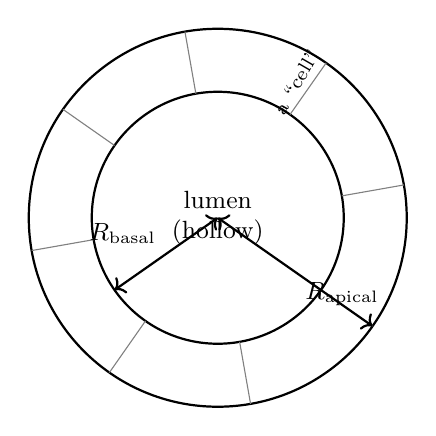
\begin{tikzpicture}[scale=1]
  % Outer cutaway circle, inner circle (lumen), a few "cell" wedges
  \def\Ro{2.4}
  \def\Ri{1.6}
  \draw[thick] (0,0) circle (\Ro);
  \draw[thick,fill=white] (0,0) circle (\Ri);
  \foreach \a in {10,55,100,145,190,235,280,325}{
    \draw[thin,gray] ({\Ro*cos(\a)},{\Ro*sin(\a)}) -- ({\Ri*cos(\a)},{\Ri*sin(\a)});
  }
  \draw[<->, thick] (0,0) -- ({\Ro*cos(-35)},{\Ro*sin(-35)})
     node[midway, below right, font=\small]{$R_{\mathrm{apical}}$};
  \draw[<->, thick] (0,0) -- ({\Ri*cos(215)},{\Ri*sin(215)})
     node[midway, above left, font=\small]{$R_{\mathrm{basal}}$};
  \node at (0,0) [font=\small, align=center] {lumen\\(hollow)};
  \node at ({2.0*cos(60)},{2.0*sin(60)}) [font=\scriptsize, rotate=60] {a ``cell''};
\end{tikzpicture}
\captionof{figure}{A cross-section through the shell. The tissue (grey
wedges) occupies a thin spherical shell between radius $R_{\mathrm{basal}}$
(inner) and $R_{\mathrm{apical}}$ (outer); the interior ($r<R_{\mathrm{basal}}$)
is completely empty -- the lumen. Nothing is modelled there at all.}
\label{fig:cross-section-cartoon}
\end{center}

Real epithelial cells are not flat polygons: they are columnar, meaning
they are noticeably taller (from the inner to the outer surface) than
they are wide, and their two ends are chemically and mechanically
different (\textbf{apical--basal polarity}). The side facing the lumen
is the \textbf{basal} side; the side facing outward (away from the
lumen, in this geometry) is the \textbf{apical} side. This project
keeps that distinction explicitly: every cell is modelled as a genuine
3D polyhedron with an apical face, a basal face, and side (``lateral'')
walls connecting them -- not a flat 2D polygon. That is why this is
called a \emph{3D} vertex model.

\section{Geometric set-up}
\label{sec:geom-setup}

\subsection{Vertex columns}

Because every cell has both an apical and a basal face, and neighbouring
cells share both, it is natural to organise the geometry around
\textbf{vertex columns}: a vertex column $j$ is a single topological
point of the tissue (a place where three cell walls meet), but it
carries \emph{two} 3D positions,
\[
  \rvec^{\mathrm{api}}_j \quad\text{(on the outer/apical surface)}, \qquad
  \rvec^{\mathrm{bas}}_j \quad\text{(on the inner/basal surface, directly ``below'' it),}
\]
which move independently under the dynamics. This is the key
simplifying assumption of the whole model: a cell's lateral wall is a
simple quadrilateral connecting corresponding apical and basal edges,
rather than an arbitrarily warped surface. It is sometimes called the
\emph{columnar} approximation, and it is standard in this kind of 3D
vertex model.

\subsection{A cell as a polyhedron}

A single cell is defined by an ordered list of vertex columns
$(j_1, j_2, \ldots, j_n)$ going around it (an $n$-sided cell). Its
boundary is made of three kinds of face:
\begin{itemize}
  \item the \textbf{apical face}: the polygon through
  $\rvec^{\mathrm{api}}_{j_1}, \ldots, \rvec^{\mathrm{api}}_{j_n}$;
  \item the \textbf{basal face}: the polygon through
  $\rvec^{\mathrm{bas}}_{j_1}, \ldots, \rvec^{\mathrm{bas}}_{j_n}$ (same
  vertex order, since apical and basal columns are paired);
  \item $n$ \textbf{lateral faces}, one per edge of the polygon: the
  quadrilateral with corners
  $\rvec^{\mathrm{api}}_{j_k}, \rvec^{\mathrm{api}}_{j_{k+1}}, \rvec^{\mathrm{bas}}_{j_{k+1}}, \rvec^{\mathrm{bas}}_{j_k}$.
\end{itemize}

\begin{center}
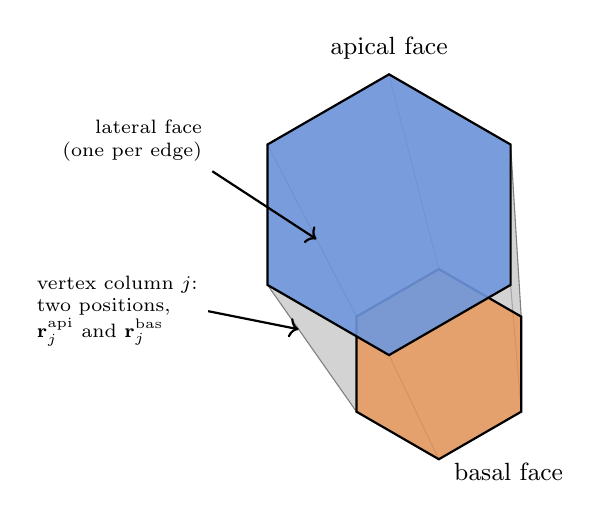
\begin{tikzpicture}[scale=1.15, every node/.style={font=\small}]
  % pseudo-3D hexagonal "wedge" cell: apical hexagon (bigger, top),
  % basal hexagon (smaller, offset down-and-right for a 3D look)
  \def\Rap{1.55}
  \def\Rbas{1.05}
  \def\shiftx{0.55}
  \def\shifty{-1.65}
  % apical hexagon vertices
  \foreach \i in {0,...,5}{
    \coordinate (A\i) at ({\Rap*cos(60*\i+90)},{\Rap*sin(60*\i+90)});
  }
  % basal hexagon vertices (shifted)
  \foreach \i in {0,...,5}{
    \coordinate (B\i) at ({\shiftx+\Rbas*cos(60*\i+90)},{\shifty+\Rbas*sin(60*\i+90)});
  }
  % lateral faces (draw first, so edges of caps sit on top)
  \foreach \i in {0,...,5}{
    \pgfmathtruncatemacro{\j}{mod(\i+1,6)}
    \fill[lateralgray, opacity=0.55] (A\i.center) -- (A\j.center) -- (B\j.center) -- (B\i.center) -- cycle;
    \draw[thin, black!50] (A\i.center) -- (B\i.center);
  }
  % basal (bottom) cap
  \fill[basalorange, opacity=0.85] (B0) \foreach \i in {1,...,5}{ -- (B\i) } -- cycle;
  \draw[thick] (B0) \foreach \i in {1,...,5}{ -- (B\i) } -- cycle;
  % apical (top) cap
  \fill[apicalblue, opacity=0.9] (A0) \foreach \i in {1,...,5}{ -- (A\i) } -- cycle;
  \draw[thick] (A0) \foreach \i in {1,...,5}{ -- (A\i) } -- cycle;

  \node[above=2pt] at (A0) {apical face};
  \node[below right=-2pt and 2pt] at (B3) {basal face};

  \draw[<-, thick] ($(A2)!0.35!(B2)$) -- ++(-1.0,0.2) node[left, align=left, font=\scriptsize] {vertex column $j$:\\ two positions,\\ $\rvec^{\mathrm{api}}_j$ and $\rvec^{\mathrm{bas}}_j$};

  \draw[<-, thick] ($(A1)!0.55!(B1)$) -- ++(-1.15,0.75) node[above left, align=right, font=\scriptsize] {lateral face\\ (one per edge)};
\end{tikzpicture}
\captionof{figure}{One cell, drawn as the hexagonal ``drum'' it really
is: an apical hexagon, a basal hexagon directly below it, and six
lateral quadrilaterals connecting corresponding edges. Every corner of
this solid is one vertex column, carrying both an apical and a basal
point.}
\label{fig:one-cell}
\end{center}

Every interior vertex column is shared by exactly three cells (it is
\textbf{trivalent}), just as three soap films always meet at $120^\circ$
along a line, and three cells in a real epithelium almost always meet
at a single junction. This is not an accident of the initial mesh: the
junction-remodelling rules in Section~\ref{sec:transitions} are
specifically designed to preserve this property.

\subsection{Building the initial mesh}
\label{sec:mesh-build}

The tissue has to start from \emph{some} tiling of the sphere into
cells. This code builds one using a classic, elegant construction:

\begin{enumerate}
  \item Start from a regular icosahedron (12 vertices, 20 triangular
  faces, 30 edges), inscribed in the unit sphere.
  \item Subdivide every triangular face into four smaller triangles
  (by adding a new point at the midpoint of every edge and pushing it
  back out onto the sphere), and repeat this $L$ times. $L$ is the one
  parameter that controls the mesh resolution (\texttt{N\_subdivision}
  in the code). Doing this exactly gives
  \[
    N_V = 10\cdot 4^{L}+2 \quad\text{vertices}, \qquad
    N_F = 20\cdot 4^{L} \quad\text{triangular faces}.
  \]
  \item Take the \textbf{dual} of this triangulation: put one cell at
  every original vertex, and give it one corner for every triangle
  touching that vertex. The corner for a triangle $(v_1,v_2,v_3)$ is
  placed along the direction $\hat{n}=\widehat{(v_2-v_1)\times(v_3-v_1)}$
  (chosen with the sign that points away from the sphere's centre);
  this is exactly the point equidistant from $v_1,v_2,v_3$, i.e.\ the
  natural circumcentre-like point for a curved (spherical) triangle. The
  apical shell is this direction scaled to radius $R_{\mathrm{apical}}$,
  and the basal shell is the very same direction scaled to
  $R_{\mathrm{basal}}$.
\end{enumerate}

Because every original icosahedron vertex has exactly 5 triangles
around it, and subdivision never changes that, this construction always
gives \textbf{exactly 12 five-sided cells} (the 12 original icosahedron
corners) and hexagonal cells everywhere else -- a geodesic, soccer-ball
(buckyball) style tiling. This is not a coincidence but a theorem
(\textbf{Euler's formula} for a sphere): for any tiling of a sphere into
$F$ polygonal faces, $E$ edges and $V$ vertices,
\begin{equation}
  V - E + F = 2 .
  \label{eq:euler}
\end{equation}
If every vertex is trivalent ($3F' = 2E$ where $F'$ is now the number of
tissue \emph{cells}, since counting sides-per-cell twice counts every
edge once from each side) and cells only ever have 5 or 6 sides, a short
bit of algebra using Eq.~\eqref{eq:euler} forces the number of
pentagons to be exactly 12, regardless of how many hexagons there are.
The code checks Eq.~\eqref{eq:euler} directly at start-up and after
every mesh change, as a cheap, powerful sanity check that nothing has
silently gone wrong with the mesh's connectivity (see
Section~\ref{sec:mod-sanity}).

\section{The energy functional}
\label{sec:energy}

Everything the tissue ``wants to do'' is encoded in a single scalar
number, the total energy $E$, which is a function of every vertex
column's two positions, $\{\rvec^{\mathrm{api}}_j, \rvec^{\mathrm{bas}}_j\}$.
The tissue evolves (Section~\ref{sec:dynamics}) by moving vertices
\emph{downhill} in this energy, i.e.\ trying to reduce $E$, in exactly
the same spirit as a ball rolling downhill on a landscape --- except
here the ``landscape'' has one dimension for every coordinate of every
vertex.

The energy used here is a standard, widely-used one, built from six
physically motivated terms -- one volume term, and one matched
apical/basal pair each for area elasticity and perimeter
contractility, plus the lateral interface term:
\begin{equation}
\begin{aligned}
  E \;=\;&
  \underbrace{\sum_{\text{cells } i} \frac{K_V}{2}\bigl(V_i - V_i^0\bigr)^2}_{\text{volume elasticity}}
  \;+\;
  \underbrace{\sum_{\text{cells } i} \frac{K_A}{2}\bigl(A_i - A_i^0\bigr)^2}_{\text{apical-area elasticity}}
  \;+\;
  \underbrace{\sum_{\text{cells } i} \frac{K_P}{2}\, P_i^2}_{\text{apical perimeter contractility}}
  \\[4pt]
  &\;+\;
  \underbrace{\sum_{\text{cells } i} \frac{K_A^{\mathrm{bas}}}{2}\bigl(A_i^{\mathrm{bas}} - A_i^{0,\mathrm{bas}}\bigr)^2}_{\text{basal-area elasticity}}
  \;+\;
  \underbrace{\sum_{\text{cells } i} \frac{K_P^{\mathrm{bas}}}{2}\, \bigl(P_i^{\mathrm{bas}}\bigr)^2}_{\text{basal perimeter contractility}}
  \;+\;
  \underbrace{\sum_{\text{edges}} \Lambda \, S_{\mathrm{lat}}}_{\text{lateral interfacial tension}} .
\end{aligned}
  \label{eq:energy}
\end{equation}
Here, for cell $i$: $V_i$ is its volume (the code variable \texttt{V}),
$A_i$ is its apical face's area (\texttt{Aapi}), $P_i$ is its apical
face's perimeter (\texttt{Papi}), and $A_i^{\mathrm{bas}}, P_i^{\mathrm{bas}}$
are the \emph{same two quantities measured on the basal face instead}
(\texttt{Abas}, \texttt{Pbas}) -- built by exactly the same
fan-triangulation/edge-sum recipe as their apical counterparts
(Section~\ref{sec:basal-reverse} explains the one twist needed for the
area term). $V_i^0, A_i^0, A_i^{0,\mathrm{bas}}$ are the cell's
\emph{target} (preferred) volume, apical area and basal area
(\texttt{V0}, \texttt{A0}, \texttt{A0\_bas}); and $S_{\mathrm{lat}}$ is
the area of one lateral (cell--cell contact) face. $K_V, K_A, K_P,
K_A^{\mathrm{bas}}, K_P^{\mathrm{bas}}, \Lambda$ are constants
(moduli) set in the parameter file, controlling how strongly each
effect matters -- note $K_A^{\mathrm{bas}}$ and $K_P^{\mathrm{bas}}$
(\texttt{K\_A\_bas}, \texttt{K\_P\_bas} in the code) are entirely
independent numbers from $K_A, K_P$: nothing forces the basal face to
behave like the apical one, though it is a common and simple choice to
set them equal (Section~\ref{sec:basal-benchmark} discusses exactly
this choice, among others, once the forces have been derived).

\begin{physbox}
\textbf{Physical meaning of each term.}
\begin{itemize}[leftmargin=1.4em]
  \item \emph{Volume elasticity}, $\tfrac{K_V}{2}(V-V^0)^2$: the cell's
  interior (mostly water and macromolecules) is close to
  incompressible, so squeezing or stretching a cell away from its
  preferred volume costs energy, growing quadratically -- exactly like
  a 3D spring.
  \item \emph{Apical/basal area elasticity}, $\tfrac{K_A}{2}(A-A^0)^2$
  and $\tfrac{K_A^{\mathrm{bas}}}{2}(A^{\mathrm{bas}}-A^{0,\mathrm{bas}})^2$:
  cells tend to maintain a preferred amount of apical (and,
  independently, basal) surface -- related to their density in the
  tissue and to the actin cortex resting at that face; deviating from
  either preferred value costs energy like a spring.
  \item \emph{Apical/basal perimeter contractility},
  $\tfrac{K_P}{2}P^2$ and $\tfrac{K_P^{\mathrm{bas}}}{2}(P^{\mathrm{bas}})^2$:
  an actomyosin ``purse-string'' running around a cell's apical (or
  basal) perimeter actively contracts, and doing so against the rest
  of the tissue costs energy proportional to (perimeter)$^2$. Note
  neither term has a target value -- shorter is always energetically
  better, unlike the area/volume terms which have a preferred value
  they resist moving away from in \emph{either} direction.
  \item \emph{Lateral interfacial tension}, $\Lambda\, S_{\mathrm{lat}}$:
  the wall between two neighbouring cells \emph{is} their contact
  surface, and it has its own effective tension, coming from the
  balance of cell--cell adhesion (which lowers the energy of contact,
  effectively $\Lambda<0$ locally) and cortical tension at that
  interface (which raises it, $\Lambda>0$ locally). One single
  coefficient $\Lambda$ is used per interface here, and its sign
  matters a great deal (Section~\ref{sec:instability} discusses what
  happens when $\Lambda$ is strongly negative).
\end{itemize}
\end{physbox}

This is the same family of energy used in essentially all modern vertex
models of epithelia; what is specific to this 3D, apical--basal version
is that $V_i$ is a true 3D polyhedron volume (not inferred from a 2D
area and a fixed height), that the tension term acts on a genuine
3D lateral wall \emph{area} $S_{\mathrm{lat}}$ (not an edge length as it
would in a 2D model), and that the apical and basal faces each carry
their own independent area/perimeter energetics rather than only the
apical face being mechanically active. A note on naming: the code
calls the lateral modulus \texttt{Lambda\_line} and this document
sometimes still calls the effect ``line tension'' in asides -- that
name is inherited from 2D vertex models, where the contact between two
cells really is a 1D edge (a line), so the term there is written
$\Lambda\cdot(\text{edge length})$. Here the corresponding contact is
a genuine 2D wall, so the same physical idea becomes
$\Lambda\cdot(\text{wall area})$, exactly as written above -- ``lateral
interfacial tension'' is the accurate name in 3D, and is preferred
throughout this document.

\subsection*{Why these six terms, and not some other combination?}
A natural question at this point: why not just give every cell a
single surface tension $\gamma$ acting on its whole boundary, the way
you would for a simple liquid droplet or a soap bubble, instead of
five separate face-by-face terms? And is the lateral term really a
separate ``adhesion'' effect on top of everything else, or is it the
same thing as cell--cell adhesion?
\begin{physbox}
\textbf{Two clarifications.}
\begin{itemize}[leftmargin=1.4em]
  \item \textbf{A cell is not mechanically uniform, so one surface
  tension is not enough.} A real epithelial cell's cortex is
  biologically different at different faces, and can be different
  again at the apical face versus the basal one -- e.g. the apical
  face often carries a prominent contractile actomyosin
  ``purse-string'' encircling the junctional belt, while the basal
  face (sitting on, or facing, something mechanically different --
  a basement membrane in a real tissue, or the lumen cavity in the
  geometries this code targets, Section~\ref{sec:geom-setup}) can have
  its own, independently tuned amount of contractility and area
  elasticity. Within a single face, the two mechanisms are also
  qualitatively different from each other: perimeter contractility
  ($\tfrac{K_P}{2}P^2$ or $\tfrac{K_P^{\mathrm{bas}}}{2}(P^{\mathrm{bas}})^2$)
  is an \emph{active} process (myosin motors pulling, whether or not
  it is energetically favourable) with no preferred length -- it only
  ever wants $P\to 0$ -- while area elasticity
  ($\tfrac{K_A}{2}(A-A^0)^2$ or its basal counterpart) is a completely
  different, \emph{passive} effect: resistance to compressing or
  stretching that face away from a preferred size, resisting changes
  in \emph{either} direction. An active, one-directional pull and a
  passive, two-directional spring cannot be captured by a single
  tension coefficient, so both terms are needed at each face -- this
  is exactly the reasoning behind the widely used 2D Farhadifar
  \emph{et al.} (2007) vertex energy, of which the apical terms here
  are a direct 3D descendant, now mirrored onto the basal face as
  well. Giving the two faces \emph{independent} moduli
  ($K_A^{\mathrm{bas}}, K_P^{\mathrm{bas}}$ separate from $K_A, K_P$)
  rather than forcing them equal is a deliberate choice: it lets you
  model anything from a perfectly symmetric apical--basal tissue
  (set them equal -- the code's own default if you omit the basal
  keys from \texttt{para.in}) to a strongly polarised one (e.g. a
  much stiffer or more contractile basal side, representing a real
  basement membrane), and to see the difference for yourself
  (Section~\ref{sec:basal-benchmark} does exactly that).
  \item \textbf{The lateral term \emph{is} cell--cell adhesion, not
  something separate from it.} $S_{\mathrm{lat}}$ in
  Eq.~\ref{eq:energy} is precisely the lateral wall shared by two
  neighbouring cells -- their actual contact surface. So
  $\Lambda\,S_{\mathrm{lat}}$ is not an extra ingredient added on top of
  adhesion; it is the adhesion energy (together with whatever cortical
  tension sits at that same junction), living exactly where you would
  expect it to, at the contact area between the two cells, as already
  explained above.
\end{itemize}
\end{physbox}

\section{Deriving the forces from the energy functional}
\label{sec:forces}

This is the heart of the physics: everything the simulation does, at
every single time step, is compute the energy $E$ of
Eq.~\ref{eq:energy} as a function of \emph{every} vertex position, and
then move every vertex a little bit downhill. This section derives,
without skipping steps, exactly how ``downhill'' is computed --
matching, line by line, what \texttt{Force.f90} actually does.

\subsection{The general principle: force = $-\partial E/\partial r$}
In overdamped mechanics (Section~\ref{sec:dynamics} explains why this
is the right regime for a cell), the force on any degree of freedom is
minus the gradient of the energy with respect to it:
\begin{equation}
  \vec F_{\vec r} = -\frac{\partial E}{\partial \vec r} .
  \label{eq:force-def}
\end{equation}
Here every apical point $\rvec_{\mathrm{api}}(j)$ and every basal point
$\rvec_{\mathrm{bas}}(j)$ (one vertex column $j$ has two of these, see
Section~\ref{sec:geom-setup}) is its own independent degree of freedom,
so we need $\partial E/\partial \rvec_{\mathrm{api}}(j)$ and
$\partial E/\partial \rvec_{\mathrm{bas}}(j)$ for \emph{every} $j$.
Since $E$ in Eq.~\ref{eq:energy} is built entirely out of volumes
$V_i$, areas $A_i$ and perimeters $P_i$, and since $E$ is just a sum
over cells, the chain rule reduces the whole problem to one question,
asked of every cell $i$ that vertex $j$ belongs to:
\emph{how does this cell's volume/area/perimeter change when I nudge
one of its corners?} The rest of this section builds up the answer
from two elementary pieces (a tetrahedron's volume and a triangle's
area) and then assembles them into whole cells exactly as the code
does.

\subsection{Building block 1: the signed volume of a tetrahedron}
\label{sec:tetra-vol}
Take the origin $O$ (the centre of the sphere) together with any three
points $\pvec, \qvec, \rvec$. They define a tetrahedron. Its volume is
the classic ``scalar triple product'' formula
\begin{equation}
  \mathrm{vol}(\pvec,\qvec,\rvec) = \frac{1}{6}\,\pvec\cdot(\qvec\times\rvec) .
  \label{eq:tetra-vol}
\end{equation}

\begin{figure}[h]
\centering
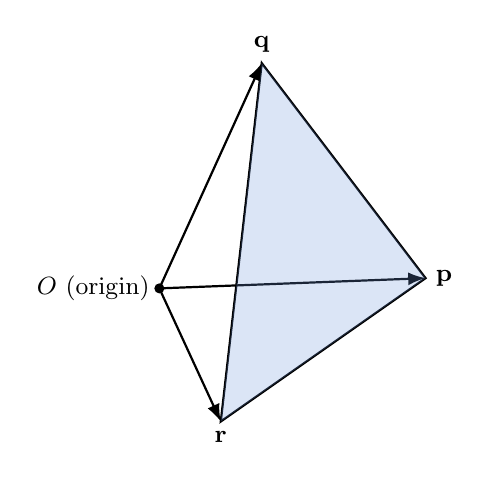
\begin{tikzpicture}[scale=1.3, every node/.style={font=\small}]
  \coordinate (O) at (0,0);
  \coordinate (P) at (2.6,0.1);
  \coordinate (Q) at (1.0,2.2);
  \coordinate (R) at (0.6,-1.3);
  \draw[-{Latex[length=2.2mm]}, thick] (O) -- (P) node[right] {$\pvec$};
  \draw[-{Latex[length=2.2mm]}, thick] (O) -- (Q) node[above] {$\qvec$};
  \draw[-{Latex[length=2.2mm]}, thick] (O) -- (R) node[below] {$\rvec$};
  \draw[thick] (P) -- (Q) -- (R) -- cycle;
  \fill[apicalblue, opacity=0.25] (P) -- (Q) -- (R) -- cycle;
  \fill (O) circle (1.4pt) node[left] {$O$ (origin)};
\end{tikzpicture}
\caption{The elementary building block: the tetrahedron formed by the
origin $O$ and three points $\pvec,\qvec,\rvec$. Its volume is
$\frac16 \pvec\cdot(\qvec\times\rvec)$, and summing this quantity over
every triangle of a closed, consistently-oriented surface (with
$\pvec,\qvec,\rvec$ always the three corners of one surface triangle)
gives the volume enclosed by that whole surface -- this is exactly how
every volume in this code is computed.}
\label{fig:tetra}
\end{figure}

\emph{Why does summing this over a closed surface give the enclosed
volume?} This is the divergence theorem in disguise. For any closed
surface $S$ enclosing a region of volume $V$, taking $\vec F(\rvec)=\rvec$
(so $\nabla\cdot\vec F = 3$) gives
\begin{equation}
  V = \frac{1}{3}\oint_S \rvec\cdot\hat n \; dA .
\end{equation}
If $S$ is triangulated into flat triangles $(\pvec,\qvec,\rvec)$, each with
consistently \emph{outward} orientation, the contribution of one
triangle to this surface integral works out to exactly
$\pvec\cdot(\qvec\times\rvec)/6$ (this is nothing but the volume of the
tetrahedron from $O$ to that triangle, signed positive when the
triangle's outward normal points away from $O$ and negative otherwise).
Crucially, this works for \emph{any} choice of the reference point
(here always the origin/sphere centre, for convenience) -- the
divergence theorem does not care where you put it, as long as the
same point is used for every triangle and the orientation is
consistent. This is exactly why the code can compute a cell's own
volume, and separately the whole lumen's volume, using the very same
formula with the very same origin, just triangulating different
surfaces.

\paragraph{Gradients.} We need
$\partial\,\mathrm{vol}/\partial\pvec$, and likewise for $\qvec,\rvec$.
Since $\pvec\cdot(\qvec\times\rvec)$ is \emph{linear} in $\pvec$ (the vector
$\qvec\times\rvec$ does not depend on $\pvec$ at all), its gradient with
respect to $\pvec$ is simply that coefficient vector:
\begin{equation}
  \frac{\partial\, \mathrm{vol}}{\partial \pvec} = \frac{\qvec\times\rvec}{6}.
\end{equation}
To get the gradients with respect to $\qvec$ and $\rvec$ we use one
standard vector identity: the scalar triple product is unchanged under
a \emph{cyclic} relabelling of its three vectors,
\begin{equation}
  \pvec\cdot(\qvec\times\rvec) \;=\; \qvec\cdot(\rvec\times\pvec) \;=\; \rvec\cdot(\pvec\times\qvec) .
  \label{eq:cyclic}
\end{equation}
(This is easiest to see by writing the triple product as the
determinant of the $3\times3$ matrix with rows $\pvec,\qvec,\rvec$: cyclically
permuting the rows of a determinant leaves it unchanged, while swapping
any two rows flips its sign.) Using the middle expression in
Eq.~\ref{eq:cyclic}, $\mathrm{vol}=\frac16\qvec\cdot(\rvec\times\pvec)$ is now
linear in $\qvec$, so by the same argument
$\partial\,\mathrm{vol}/\partial\qvec = (\rvec\times\pvec)/6$; and from the
rightmost expression, $\partial\,\mathrm{vol}/\partial\rvec=(\pvec\times\qvec)/6$.
Collecting all three:
\begin{equation}
  \frac{\partial\, \mathrm{vol}}{\partial \pvec} = \frac{\qvec\times\rvec}{6}, \qquad
  \frac{\partial\, \mathrm{vol}}{\partial \qvec} = \frac{\rvec\times\pvec}{6}, \qquad
  \frac{\partial\, \mathrm{vol}}{\partial \rvec} = \frac{\pvec\times\qvec}{6}.
  \label{eq:tetra-grad}
\end{equation}
These are \emph{exact} (no approximation, no finite differences) and
this is precisely \texttt{tetra\_vol\_grad} in \texttt{mod\_geometry.f90}:

\begin{lstlisting}
pure subroutine tetra_vol_grad(p, q, r, vol, gp, gq, gr)
  real(dp), intent(in)  :: p(3), q(3), r(3)
  real(dp), intent(out) :: vol, gp(3), gq(3), gr(3)
  vol = dot_product(p, cross(q, r)) / 6.0_dp
  gp  = cross(q, r) / 6.0_dp
  gq  = cross(r, p) / 6.0_dp
  gr  = cross(p, q) / 6.0_dp
end subroutine tetra_vol_grad
\end{lstlisting}

\subsection{Building block 2: the area of a triangle}
\label{sec:tri-area}
For a triangle with corners $\pvec,\qvec,\rvec$, form the (non-unit) normal
vector and its length,
\begin{equation}
  \vec n = (\qvec-\pvec)\times(\rvec-\pvec), \qquad
  A = \tfrac12 |\vec n|, \qquad
  \hat n = \vec n / |\vec n| .
\end{equation}
To differentiate $A$ with respect to $\pvec$, first recall the general
fact that for any vector $\vec n(\pvec)$, a small change $d\pvec$ produces
$d|\vec n| = \hat n \cdot d\vec n$ (the change in a vector's \emph{length}
is the component of its change \emph{along its own direction} -- this
is just $|\vec n|=\sqrt{\vec n\cdot\vec n}$ differentiated). So
\begin{equation}
  dA = \tfrac12\, \hat n \cdot d\vec n .
  \label{eq:dA}
\end{equation}
Now compute $d\vec n$ for a small displacement $d\pvec$ of the corner
$\pvec$ only (holding $\qvec,\rvec$ fixed):
\begin{align}
  d\vec n &= d\bigl[(\qvec-\pvec)\times(\rvec-\pvec)\bigr]
          = (-d\pvec)\times(\rvec-\pvec) + (\qvec-\pvec)\times(-d\pvec) \notag\\
          &= -d\pvec\times(\rvec-\pvec) - (\qvec-\pvec)\times d\pvec
           = -d\pvec\times(\rvec-\pvec) + d\pvec\times(\qvec-\pvec) \notag\\
          &= d\pvec\times\bigl[(\qvec-\pvec)-(\rvec-\pvec)\bigr]
           = d\pvec\times(\qvec-\rvec),
  \label{eq:dn}
\end{align}
where we used $\vec a\times\vec b=-\vec b\times \vec a$ to flip the second
cross product. Substituting Eq.~\ref{eq:dn} into Eq.~\ref{eq:dA},
\begin{equation}
  dA = \tfrac12\, \hat n \cdot \bigl[d\pvec\times(\qvec-\rvec)\bigr] .
\end{equation}
To read off the gradient we need $d\pvec$ standing alone in a dot
product with $dA$; the cyclic identity Eq.~\ref{eq:cyclic} lets us move
it there: $\hat n\cdot(d\pvec\times(\qvec-\rvec)) = d\pvec\cdot\bigl[(\qvec-\rvec)\times\hat n\bigr]$.
So
\begin{equation}
  \frac{\partial A}{\partial \pvec} = \tfrac12 (\qvec-\rvec)\times\hat n
  = \tfrac12\, \hat n\times(\rvec-\qvec),
\end{equation}
(the second form follows from antisymmetry of the cross product, and
is the form used in the code). Relabelling the same argument for
$\qvec$ and $\rvec$ in turn (the triangle's three corners play exactly
symmetric roles in this derivation) gives all three gradients:
\begin{equation}
  \frac{\partial A}{\partial \pvec} = \tfrac12\, \hat n\times(\rvec-\qvec), \qquad
  \frac{\partial A}{\partial \qvec} = \tfrac12\, \hat n\times(\pvec-\rvec), \qquad
  \frac{\partial A}{\partial \rvec} = \tfrac12\, \hat n\times(\qvec-\pvec).
  \label{eq:tri-grad}
\end{equation}
Two useful checks, both exploited in \texttt{sanity\_checks.f90}: (i)
each gradient lies in the plane of the triangle and is perpendicular to
the \emph{opposite} edge, which matches the intuition that pushing a
corner directly away from the opposite side grows the area fastest;
(ii) adding all three gradients gives
$\hat n\times[(\rvec-\qvec)+(\pvec-\rvec)+(\qvec-\pvec)]=\hat n\times\vec 0=\vec 0$,
i.e. sliding the \emph{whole} triangle rigidly changes its area by
zero, as it must. This is \texttt{tri\_area\_grad}:

\begin{lstlisting}
pure subroutine tri_area_grad(p, q, r, area, gp, gq, gr, nhat_out)
  n   = cross(q - p, r - p)
  nrm = norm3(n);  nhat = n / nrm;  area = 0.5_dp * nrm
  gp = 0.5_dp * cross(nhat, r - q)
  gq = 0.5_dp * cross(nhat, p - r)
  gr = 0.5_dp * cross(nhat, q - p)
end subroutine tri_area_grad
\end{lstlisting}

\subsection{From one triangle to a whole cell: fan triangulation}
\label{sec:fan}
A cell's apical face is not a triangle -- it is an $n$-sided polygon
(recall Section~\ref{sec:mesh-build}: mostly hexagons, twelve
pentagons). To reuse the two exact building blocks above, the code
cuts every polygon face into triangles by \emph{fanning out from the
cell's own centroid} $\ca = \tfrac1n\sum_{k=1}^n \Aarr_k$ (the plain
average of that cell's $n$ apical corners, \texttt{ca} in the code) --
one triangle $(\ca, \Aarr_k, \Aarr_{k+1})$ for every one of the $n$
edges, wrapping around ($k{+}1$ meaning ``back to 1'' after $k=n$).

\begin{figure}[h]
\centering
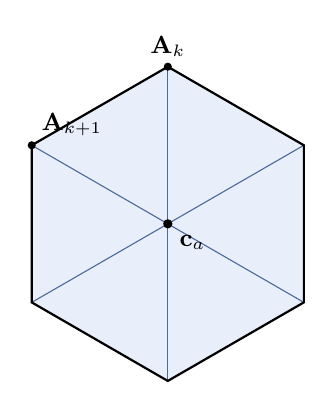
\begin{tikzpicture}[scale=1.05, every node/.style={font=\small}]
  \def\R{1.9}
  \foreach \i in {0,...,5} {
    \coordinate (V\i) at ({90+\i*60}:\R);
  }
  \coordinate (C) at (0,0);
  \foreach \i in {0,...,5} {
    \pgfmathtruncatemacro{\j}{mod(\i+1,6)}
    \fill[apicalblue, opacity=0.15] (C) -- (V\i) -- (V\j) -- cycle;
    \draw[apicalblue!70!black] (C) -- (V\i);
  }
  \draw[thick] (V0) \foreach \i in {1,...,5} { -- (V\i) } -- cycle;
  \fill (C) circle (1.6pt) node[below right=1pt] {$\ca$};
  \fill (V0) circle (1.4pt) node[above] {$\Aarr_k$};
  \fill (V1) circle (1.4pt) node[above right] {$\Aarr_{k+1}$};
\end{tikzpicture}
\caption{Fan triangulation of a hexagonal apical face from its own
centroid $\ca$: one triangle $(\ca,\Aarr_k,\Aarr_{k+1})$ per edge. The
cell's apical area and its contribution to the cell's volume are both
computed by summing Eqs.~\ref{eq:tetra-vol} and~\ref{eq:tri-grad} over
exactly these triangles.}
\label{fig:fan}
\end{figure}

Summing the tetrahedron-volume of Eq.~\ref{eq:tetra-vol} over all $n$
fan triangles $(\ca,\Aarr_k,\Aarr_{k+1})$ gives the volume swept out
by the apical cap (as part of the divergence-theorem sum explained in
Section~\ref{sec:tetra-vol}); summing the triangle-area of
Eq.~\ref{eq:tri-grad} over the same $n$ triangles gives the total
apical area $A_{\mathrm{api}} = \sum_k \mathrm{area}(\ca,\Aarr_k,\Aarr_{k+1})$.
The basal cap is fanned from its own centroid $\cb$ in exactly the
same way (Section~\ref{sec:basal-reverse} explains the one twist:
the triangle order is reversed there).

\subsection{The centroid chain rule -- the one subtle step}
\label{sec:centroid-chain}
Here is the step that is easy to get wrong, and the reason this
section exists in this much detail: $\ca$ is not an independent point.
It is built from \emph{every} corner of the polygon,
$\ca = \tfrac1n\sum_{i=1}^n \Aarr_i$. So when we ask how the apical
cap's volume changes as we move \emph{one particular} corner
$\Aarr_j$, that corner's motion affects the sum in two separate ways:
\begin{enumerate}
  \item \textbf{Directly}: $\Aarr_j$ is an explicit corner of exactly
  two fan triangles -- the one where $k=j$ (there it plays the role of
  the \emph{second} argument, $\qvec$, of \texttt{tetra\_vol\_grad}) and
  the one where $k{+}1=j$, i.e. $k=j-1$ (there it plays the role of the
  \emph{third} argument, $\rvec$).
  \item \textbf{Indirectly, through the centroid}: moving $\Aarr_j$ by
  $d\Aarr_j$ shifts \emph{every} fan triangle's apex $\ca$ by
  $\partial \ca/\partial \Aarr_j \cdot d\Aarr_j = \tfrac1n\, d\Aarr_j$
  (a $\tfrac1n$ nudge of the centroid for every single one of the $n$
  triangles, since $\ca$ is a plain average).
\end{enumerate}
The total derivative is the sum of both contributions, added up over
\emph{every} triangle $k=1,\dots,n$ in the fan (the chain rule, applied
term by term):
\begin{equation}
  \frac{\partial V_{\mathrm{api\ cap}}}{\partial \Aarr_j}
  = \underbrace{\left.\frac{\partial\, \mathrm{vol}_k}{\partial \Aarr_j}\right|_{k=j} }_{\text{direct, as } \qvec}
  \;+\;
  \underbrace{\left.\frac{\partial\, \mathrm{vol}_k}{\partial \Aarr_j}\right|_{k=j-1}}_{\text{direct, as } \rvec}
  \;+\;
  \frac{1}{n}\sum_{k=1}^{n} \frac{\partial\, \mathrm{vol}_k}{\partial \ca} ,
  \label{eq:chain-rule}
\end{equation}
with $\mathrm{vol}_k \equiv \mathrm{vol}(\ca,\Aarr_k,\Aarr_{k+1})$ and each
piece on the right read straight off Eq.~\ref{eq:tetra-grad}
($\partial\,\mathrm{vol}_k/\partial\ca$ is the ``$\pvec$'' gradient there,
since $\ca$ occupies the first argument slot). This is exactly the
triple loop in \texttt{Force.f90}:

\begin{lstlisting}
do k = 1, n
  kp = mod(k, n) + 1
  call tetra_vol_grad(ca, Aarr(:,k), Aarr(:,kp), vtri, gp, gq, gr)
  V = V + vtri
  gV_A(:, k)  = gV_A(:, k)  + gq        ! direct, A_k as "q"
  gV_A(:, kp) = gV_A(:, kp) + gr        ! direct, A_kp as "r"
  do j = 1, n
    gV_A(:, j) = gV_A(:, j) + gp / real(n, dp)   ! indirect, via centroid
  end do
end do
\end{lstlisting}
The inner \texttt{do j = 1, n} loop is exactly the $\tfrac1n\sum_k(\cdot)$
term of Eq.~\ref{eq:chain-rule}: every triangle's $\pvec$-gradient
(its contribution through the centroid) gets smeared out, with weight
$1/n$, onto \emph{every} vertex of the polygon -- not just the two
corners of that one triangle. The apical-area gradient
(\texttt{gArea\_A}) is built by the identical two-part logic, just
using \texttt{tri\_area\_grad} in place of \texttt{tetra\_vol\_grad}.

\subsection{The basal cap: same trick, reversed winding}
\label{sec:basal-reverse}
The basal cap is fanned from its own centroid $\cb$ exactly as above,
\emph{except} the two non-centroid corners are swapped:
$(\cb,\Barr_{k+1},\Barr_k)$ instead of $(\cb,\Barr_k,\Barr_{k+1})$. Why
the flip? A closed polyhedron's volume (Section~\ref{sec:tetra-vol})
only comes out right if \emph{every} face of that polyhedron is
triangulated with a consistently \emph{outward}-pointing orientation.
The apical fan, with its particular corner order, already has an
outward normal (pointing away from the cell, out towards $R_{\mathrm{api}}$).
But the basal cap is the \emph{opposite} face of the same cell -- its
outward normal must point the other way, further inward, away from the
cell's own interior and into the lumen. Swapping two corners of every
triangle flips its normal, which is exactly the fix needed:

\begin{figure}[h]
\centering
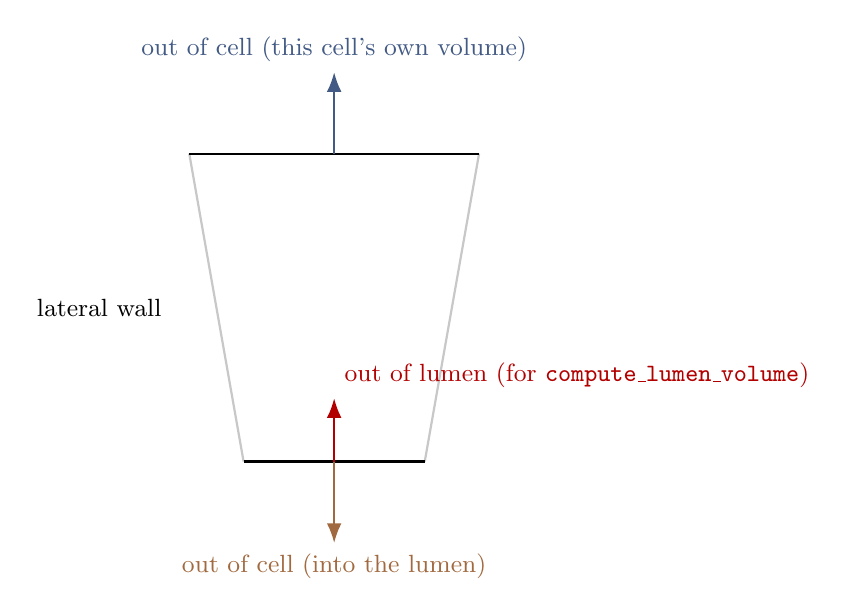
\begin{tikzpicture}[scale=1.15, every node/.style={font=\small}]
  \coordinate (A1) at (-1.6,1.7);
  \coordinate (A2) at (1.6,1.7);
  \coordinate (B1) at (-1.0,-1.7);
  \coordinate (B2) at (1.0,-1.7);
  \coordinate (Ca) at (0,1.7);
  \coordinate (Cb) at (0,-1.7);
  \fill[apicalblue, opacity=0.25] (A1) -- (A2) -- (Ca) -- cycle;
  \fill[basalorange, opacity=0.3] (B1) -- (B2) -- (Cb) -- cycle;
  \draw[lateralgray, thick] (A1) -- (B1);
  \draw[lateralgray, thick] (A2) -- (B2);
  \draw[thick] (A1) -- (A2);
  \draw[thick] (B1) -- (B2);
  \draw[-{Latex[length=2.5mm]}, thick, apicalblue!60!black] (Ca) -- ++(0,0.9) node[above] {out of cell (this cell's own volume)};
  \draw[-{Latex[length=2.5mm]}, thick, basalorange!70!black] (Cb) -- ++(0,-0.9) node[below] {out of cell (into the lumen)};
  \draw[-{Latex[length=2.5mm]}, thick, red!70!black] (Cb) -- ++(0,0.7) node[above right, text=red!70!black] {out of lumen (for \texttt{compute\_lumen\_volume})};
  \node[left] at (-1.8,0) {lateral wall};
\end{tikzpicture}
\caption{Why the basal fan is reversed. Seen from the cell's own
interior (blue arrow), the basal face's outward normal points further
inward, into the lumen -- the opposite direction from the apical
face's outward normal. But the very same physical surface, seen from
the lumen's side (red arrow), needs the \emph{opposite} outward
direction again -- so \texttt{compute\_lumen\_volume} triangulates the
basal points in the \emph{non}-reversed order, exactly undoing the flip
used inside \texttt{compute\_forces}.}
\label{fig:basal-flip}
\end{figure}

\begin{lstlisting}
! ---- basal cap: fan from cb, REVERSED order -----------------------
do k = 1, n
  kp = mod(k, n) + 1
  call tetra_vol_grad(cb, Barr(:,kp), Barr(:,k), vtri, gp, gq, gr)
  ! ...accumulated into gV_B exactly as for the apical cap...
end do
\end{lstlisting}

\subsection{The basal area and basal perimeter}
\label{sec:basal-area-perim}
The energy functional (Eq.~\ref{eq:energy}) also has a basal-area
elasticity term and a basal perimeter contractility term, mirroring
the apical ones exactly. Both are built from the very same basal fan
used above for the volume -- with one pleasant simplification: unlike
the \emph{signed volume}, the (unsigned) triangle \emph{area} and its
gradient (Eqs.~\ref{eq:tri-grad}) do \textbf{not} depend on the order
in which the three corners are given. Swapping two corners flips the
sign of the normal $\hat n$ used inside \texttt{tri\_area\_grad} (since
$\vec n=(\qvec-\pvec)\times(\rvec-\pvec)$ changes sign when $\qvec$
and $\rvec$ are exchanged), but every gradient formula in
Eq.~\ref{eq:tri-grad} pairs $\hat n$ with a vector built from
\emph{that same} swap (e.g.\ $\hat n\times(\rvec-\qvec)$), so the two
sign flips cancel exactly, leaving the physical gradient (matched to
each actual vertex, not to its ``$\pvec$/$\qvec$/$\rvec$'' argument
slot) unchanged. In short: \emph{area doesn't care about winding, only
signed volume does} -- so the same $(\cb,\Barr_{kp},\Barr_k)$ triangle
order already used above for the reversed-winding volume fan can be
reused as-is for the basal area and perimeter, with no separate pass
and no second reversed/non-reversed distinction to track:
\begin{lstlisting}
! (continuing the same k-loop as the basal-volume fan above)
call tri_area_grad(cb, Barr(:,kp), Barr(:,k), atri, gp, gq, gr)
Abas = Abas + atri
gArea_B(:, kp) = gArea_B(:, kp) + gq
gArea_B(:, k)  = gArea_B(:, k)  + gr
do j = 1, n
  gArea_B(:, j) = gArea_B(:, j) + gp / real(n, dp)   ! same centroid chain rule as gArea_A
end do

d = Barr(:, kp) - Barr(:, k)
edge_len = norm3(d)
Pbas = Pbas + edge_len
gPer_B(:, k)  = gPer_B(:, k)  - d / edge_len          ! same recipe as the apical perimeter
gPer_B(:, kp) = gPer_B(:, kp) + d / edge_len
\end{lstlisting}
The basal-area gradient goes through exactly the same
direct-plus-centroid-chain-rule split as the apical one
(Section~\ref{sec:centroid-chain}), and the basal-perimeter gradient is
exactly the plain edge-length gradient derived just below for the
apical perimeter (Section~\ref{sec:apical-perim}), evaluated on the
basal points instead. So the basal cap ends up contributing to three things: the
cell's volume $V$ (via the reversed tetrahedron fan above), its basal
area $A_{\mathrm{bas}}$, and its basal perimeter $P_{\mathrm{bas}}$
(both via this same fan, in the same triangle order, at essentially no
extra cost).

\subsection{The lateral walls}
\label{sec:lateral-walls}
Each of the $n$ lateral faces is the quadrilateral
$(\Aarr_k,\Barr_k,\Barr_{k+1},\Aarr_{k+1})$ joining one apical edge to the
basal edge directly below it. A quadrilateral is not necessarily flat,
so the code splits it, along a fixed diagonal, into exactly two
triangles, $(\Aarr_k,\Barr_k,\Barr_{k+1})$ and
$(\Aarr_k,\Barr_{k+1},\Aarr_{k+1})$ -- no centroid involved here, so
\emph{no} chain-rule complication: each triangle's three corners are
real vertex columns, and Eqs.~\ref{eq:tetra-grad} and~\ref{eq:tri-grad}
apply directly, contributing straight into the volume-gradient and
lateral-area-gradient arrays of whichever four vertex columns
($\Aarr_k,\Barr_k,\Barr_{k+1},\Aarr_{k+1}$) happen to be the corners.
Both triangles' tetrahedron-volumes add to the cell's total volume $V$
(they are simply two more faces in the divergence-theorem sum), and
both triangles' areas add to $S_{\mathrm{lat}}$ for that one edge.

\subsection{The apical perimeter}
\label{sec:apical-perim}
The apical perimeter needs no new machinery at all: it is just the sum
of the $n$ edge lengths, $P_{\mathrm{api}}=\sum_k |\Aarr_{k+1}-\Aarr_k|$.
Writing $\vec d = \Aarr_{k+1}-\Aarr_k$ and using the same
``derivative-of-a-length'' fact as Eq.~\ref{eq:dA} ($d|\vec d| = \hat
d\cdot d\vec d$),
\begin{equation}
  \frac{\partial |\vec d|}{\partial \Aarr_k} = -\hat d, \qquad
  \frac{\partial |\vec d|}{\partial \Aarr_{k+1}} = +\hat d, \qquad \hat d = \vec d/|\vec d|,
\end{equation}
which is exactly \texttt{gPer\_A(:,k) -= d/edge\_len} and
\texttt{gPer\_A(:,kp) += d/edge\_len} in the code.

\subsection{Putting it all together: the total force}
\label{sec:force-assembly}
Every cell's volume $V$, apical area $A_{\mathrm{api}}$, apical
perimeter $P_{\mathrm{api}}$, basal area $A_{\mathrm{bas}}$, basal
perimeter $P_{\mathrm{bas}}$, and, for every one of its edges, lateral
area $S_{\mathrm{lat}}$, are now known, together with the gradient of
each with respect to every one of that cell's own vertex columns
(arrays \texttt{gV\_A}/\texttt{gV\_B}, \texttt{gArea\_A}/\texttt{gArea\_B},
\texttt{gPer\_A}/\texttt{gPer\_B}, \texttt{gLat\_A}/\texttt{gLat\_B} in
the code). Since $E$ (Eq.~\ref{eq:energy}) is a sum over cells of
simple functions of these quantities, the chain rule gives, for one
cell $i$ and one of its vertex columns $j$:
\begin{align}
  \frac{\partial E_i}{\partial \Aarr_j} &=
     K_V\underbrace{(V_i-V_i^0)}_{\Delta V}\frac{\partial V_i}{\partial \Aarr_j}
   + K_A\underbrace{(A_i-A_i^0)}_{\Delta A}\frac{\partial A_i}{\partial \Aarr_j}
   + K_P P_i \frac{\partial P_i}{\partial \Aarr_j}
   + \tfrac12\Lambda\frac{\partial S_{\mathrm{lat},i}}{\partial \Aarr_j}, \label{eq:dE-api}\\
  \frac{\partial E_i}{\partial \Barr_j} &=
     K_V\Delta V\,\frac{\partial V_i}{\partial \Barr_j}
   + K_A^{\mathrm{bas}}\underbrace{(A_i^{\mathrm{bas}}-A_i^{0,\mathrm{bas}})}_{\Delta A^{\mathrm{bas}}}\frac{\partial A_i^{\mathrm{bas}}}{\partial \Barr_j}
   + K_P^{\mathrm{bas}} P_i^{\mathrm{bas}} \frac{\partial P_i^{\mathrm{bas}}}{\partial \Barr_j}
   + \tfrac12\Lambda\frac{\partial S_{\mathrm{lat},i}}{\partial \Barr_j}, \label{eq:dE-bas}
\end{align}
using $\partial/\partial V[(K_V/2)(V-V^0)^2] = K_V(V-V^0)$ and
likewise for the $K_A$, $K_P$, $K_A^{\mathrm{bas}}$ and
$K_P^{\mathrm{bas}}$ terms (elementary calculus on a quadratic; the two
perimeter terms are the $A^0\to 0$-less special case, i.e. just
$\partial/\partial P[(K_P/2)P^2]=K_PP$). Notice how closely
Eq.~\ref{eq:dE-bas} mirrors Eq.~\ref{eq:dE-api} -- $\Barr_j$ now feeds
into $V_i$, $A_i^{\mathrm{bas}}$, $P_i^{\mathrm{bas}}$ and
$S_{\mathrm{lat},i}$, exactly the basal-face counterparts of what
$\Aarr_j$ feeds into on the apical side. The factor $\tfrac12$ on the
lateral term is there because \emph{both} of the two cells sharing
that wall run this same loop over ``their own'' copy of the edge; each
contributing half means the two together contribute the full
$\Lambda\,S_{\mathrm{lat}}$ exactly once, not twice -- no such factor is
needed for the area/perimeter terms since an apical or basal face
belongs to exactly one cell, never shared between two.

Finally, summing Eqs.~\ref{eq:dE-api}--\ref{eq:dE-bas} over every cell
$i$ that owns vertex column $j$ (a vertex is shared by 2--3 cells) and
negating (Eq.~\ref{eq:force-def}) gives the actual force used to move
the vertex:
\begin{equation}
  \boxed{
  \fapi{j} = -\sum_{i \ni j}\frac{\partial E_i}{\partial \Aarr_j}, \qquad
  \fbas{j} = -\sum_{i \ni j}\frac{\partial E_i}{\partial \Barr_j}
  }
  \label{eq:final-force}
\end{equation}
which is precisely the accumulation step at the end of the \texttt{do
ic = 1, n\_cell} loop in \texttt{compute\_forces}:
\begin{lstlisting}
f_api(:, gvid) = f_api(:, gvid) - ( K_V * dV * gV_A(:, k)          &
                                  + K_A * dA * gArea_A(:, k)       &
                                  + K_P * Papi * gPer_A(:, k)      &
                                  + 0.5_dp * Lambda_line * gLat_A(:, k) )
f_bas(:, gvid) = f_bas(:, gvid) - ( K_V * dV * gV_B(:, k)          &
                                  + K_A_bas * dAbas * gArea_B(:, k) &
                                  + K_P_bas * Pbas * gPer_B(:, k)   &
                                  + 0.5_dp * Lambda_line * gLat_B(:, k) )
\end{lstlisting}
Because the code loops over cells (not over vertices), and every cell
adds its own contribution \emph{onto} whatever is already in
\texttt{f\_api(:,gvid)}/\texttt{f\_bas(:,gvid)} for each of its corners
(rather than overwriting), a vertex shared by three cells automatically
ends up with the sum of all three cells' pulls on it -- exactly the sum
in Eq.~\ref{eq:final-force}. Every one of these gradients is exact and
analytic (no finite differences anywhere in the production code);
\texttt{sanity\_checks.f90}'s \texttt{test\_geometry\_gradients} checks
Eqs.~\ref{eq:tetra-grad} and~\ref{eq:tri-grad} against numerical finite
differences at start-up, and \texttt{test\_cube\_volume} checks the
whole pipeline above (fan triangulation, reversed basal winding,
lateral splitting, all of it) against an exact unit cube, before any
simulation is trusted.

\section{Overdamped Langevin dynamics}
\label{sec:dynamics}

Section~\ref{sec:forces} gave us, at any instant, the force
$\fapi{j}$ and $\fbas{j}$ on every vertex. This section is about what
the code does with that force: how positions actually move over time.

\subsection{Why ``overdamped''?}
A cell is enormous compared to a molecule but tiny compared to
everyday objects, and it lives in a thick, sticky, watery environment.
The relevant physics here is \emph{low Reynolds number} motion: viscous
(drag) forces completely dominate over inertia. If you stopped pushing
a bacterium (or a vertex in this model), it would not coast to a stop
over some time later like a car easing off the accelerator -- it would
stop \emph{immediately}, because drag is so overwhelmingly larger than
any inertial term $m\,\ddot{\rvec}$. This is why the equation of motion
used here has \emph{no} acceleration term at all -- it is first-order
in time, not second-order like Newton's law:
\begin{equation}
  \zeta \,\frac{d\rvec}{dt} = -\frac{\partial E}{\partial \rvec} + \boldsymbol{\xi}(t),
  \label{eq:langevin}
\end{equation}
applied independently to every $\rvec_{\mathrm{api}}(j)$ and
$\rvec_{\mathrm{bas}}(j)$. Here $\zeta$ (\texttt{zeta\_friction}) is a
drag/friction coefficient (how strongly the surrounding medium resists
a vertex's motion), $-\partial E/\partial\rvec$ is exactly the force
derived in Section~\ref{sec:forces}, and $\boldsymbol\xi(t)$ is a
random ``thermal'' force representing every microscopic jiggling
effect the model does not resolve explicitly (molecular collisions,
noisy biochemical activity, and so on).

\subsection{The noise term, and why its size is not arbitrary}
$\boldsymbol\xi(t)$ is not just ``some noise'' -- its strength is fixed
by the \emph{fluctuation--dissipation theorem}: whatever mechanism
damps motion (here, friction $\zeta$) must also be the source of
random kicks, in a fixed ratio set by the temperature, otherwise the
system would not settle to the correct thermal equilibrium. This fixes
the noise's statistics to
\begin{equation}
  \langle \xi_a(t)\,\xi_b(t')\rangle = 2\,\zeta\, k_BT\, \delta_{ab}\,\delta(t-t'),
\end{equation}
i.e. it is uncorrelated between different Cartesian components $a,b$
and between different times, and its overall size grows with both the
friction $\zeta$ and the effective temperature $k_BT$
(\texttt{kBT} in the parameter file -- here best read as an
\emph{effective} noise strength standing in for all unresolved
biological fluctuations, not necessarily a literal thermodynamic
temperature).

\subsection{Discretising: the Euler--Maruyama scheme}
The simulation cannot integrate Eq.~\ref{eq:langevin} exactly, so it
takes small time steps $dt$ (\texttt{dt}) and updates every position by
\begin{equation}
  \rvec(t+dt) = \rvec(t) + \frac{dt}{\zeta}\, \vec F(t)
  \;+\; \sqrt{\frac{2k_BT\,dt}{\zeta}}\; \mathcal N(0,1),
  \label{eq:euler-maruyama}
\end{equation}
independently for each of the 3 spatial components, and independently
for every apical and every basal point. The first two terms are just
forward-Euler integration of $\zeta\,d\rvec/dt = \vec F$. The noise
amplitude in the last term follows directly from the
fluctuation-dissipation relation above: over one step of size $dt$,
integrating white noise with the correlation above gives a random
displacement that is Gaussian with mean zero and variance
$2k_BT\,dt/\zeta$ per component -- taking the square root gives exactly
the coefficient of the standard-normal draw $\mathcal N(0,1)$ used in
Eq.~\ref{eq:euler-maruyama}. This particular way of discretising a
Langevin equation is called \emph{Euler--Maruyama}: forward Euler for
the deterministic (force) part, plus one freshly drawn random number
per step for the stochastic part.

This is implemented directly in \texttt{Langevin\_update.f90}:
\begin{lstlisting}
subroutine langevin_step()
  coef      = dt / zeta_friction
  noise_amp = sqrt(2.0_dp * kBT * dt / zeta_friction)
  do i = 1, n_vert
    if (.not. vert_alive(i)) cycle
    do d = 1, 3
      r_api(d, i) = r_api(d, i) + coef * f_api(d, i) + noise_amp * gaussian_rand()
      r_bas(d, i) = r_bas(d, i) + coef * f_bas(d, i) + noise_amp * gaussian_rand()
    end do
  end do
end subroutine langevin_step
\end{lstlisting}
A fresh independent \texttt{gaussian\_rand()} draw is used for every
single one of the 3 components of every one of the (up to) two points
per vertex column, matching the $\delta_{ab}$ (uncorrelated components)
in the fluctuation-dissipation relation above. \texttt{gaussian\_rand}
itself turns MATLAB/Fortran's built-in uniform random numbers into
Gaussian ones via the standard Box--Muller transform,
$g=\sqrt{-2\ln u_1}\,\cos(2\pi u_2)$ for two independent uniform
draws $u_1,u_2\in(0,1)$ -- a standard trick, not specific to this
model. Setting $k_BT=0$ switches off the noise term entirely
(\texttt{noise\_amp} becomes exactly zero), giving pure deterministic
energy-minimising relaxation -- useful for testing the mechanics in
isolation from thermal fluctuations.

\section{Topological transitions: T1, T2, and cell division}
\label{sec:transitions}

Section~\ref{sec:dynamics}'s Langevin update moves vertices
\emph{continuously}. But real tissues do more than that: cells swap
neighbours as they squeeze past each other, cells are extruded/die, and
cells grow and divide. Each of these changes the tissue's
\emph{topology} -- which cells border which -- something a purely
continuous update to vertex positions can never do by itself. The code
checks for all three, periodically (every \texttt{it\_topology\_check}
steps for T1/T2, every \texttt{it\_division\_check} steps for
division), by scanning simple geometric criteria (an edge's length, a
triangular cell's area, a cell's volume) and performing explicit,
discrete ``ring surgery'' on the data structure whenever a threshold is
crossed. All three transitions follow one shared design rule, worth
stating up front: \textbf{every mutation is fully validated before
anything is changed}. Side counts, capacity limits, and geometric
sanity are all checked using only read-only queries first; only once
every check has passed does the code touch \texttt{cells(:)\%vlist} or
the vertex arrays. This means a rejected transition never leaves the
mesh half-modified -- either it happens completely and correctly, or it
does not happen at all (and every batch of transitions is followed by
an Euler-characteristic check and a full ring-integrity check, as an
independent runtime confirmation that this atomicity held).

\subsection{T1: neighbour exchange (intercalation)}
\label{sec:T1}
\textbf{Biology.} Cells in a real tissue are not stuck in one fixed
arrangement of neighbours forever -- they actively rearrange, sliding
past each other to change who touches whom. This process,
\emph{intercalation}, is one of the main ways tissues change shape
without changing the number or size of their cells, and it is a major
driver of large-scale tissue movements such as convergent extension in
early development.

\textbf{The trivalent-vertex rule.} In a proper vertex-model mesh,
every interior vertex column is shared by exactly 3 cells (this was
already built into the initial mesh in Section~\ref{sec:mesh-build},
and is checked continuously at runtime). A T1 event is the elementary
move that preserves this rule while still changing who neighbours whom.

\textbf{The set-up.} Consider an apical edge $(j,k)$, shared by two
cells $A$ and $B$. Because $j$ and $k$ are each trivalent, there is
exactly one more cell at $j$ besides $A,B$ -- call it $C$ -- and one
more at $k$ -- call it $D$. When this edge's length drops below
\texttt{L\_T1\_threshold}, the code performs the standard T1 flip.

Before looking at the flip itself, it helps to see these four cells as
what they really are: genuine 3D vertex columns, each with its own
apical and basal point, not flat 2D tiles.

\begin{figure}[h]
\centering
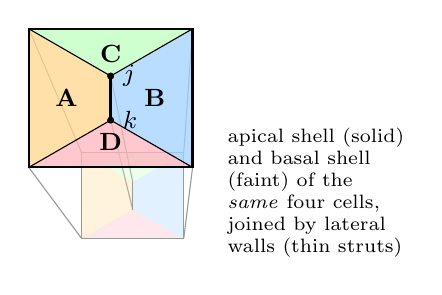
\begin{tikzpicture}[scale=0.8, every node/.style={font=\small}]
  % apical (top/outer) points -- identical to the "before" panel of
  % Fig.~\ref{fig:T1} below
  \coordinate (j) at (0,0.35);
  \coordinate (k) at (0,-0.35);
  \coordinate (NW) at (-1.3,1.1);
  \coordinate (NE) at (1.3,1.1);
  \coordinate (SW) at (-1.3,-1.1);
  \coordinate (SE) at (1.3,-1.1);
  % basal (bottom/inner) echo of the very same points: scaled down and
  % shifted, exactly the pseudo-3D convention of Fig.~\ref{fig:one-cell}
  \coordinate (jB) at (0.35,-1.33);
  \coordinate (kB) at (0.35,-1.77);
  \coordinate (NWB) at (-0.46,-0.87);
  \coordinate (NEB) at (1.16,-0.87);
  \coordinate (SWB) at (-0.46,-2.23);
  \coordinate (SEB) at (1.16,-2.23);
  % lateral walls (struts), drawn first so everything else sits on top
  \draw[thin, black!40] (NW)--(NWB) (NE)--(NEB) (SW)--(SWB) (SE)--(SEB) (j)--(jB) (k)--(kB);
  % basal shell (faint)
  \fill[cellB, opacity=0.3] (jB) -- (NEB) -- (SEB) -- (kB) -- cycle;
  \fill[cellA, opacity=0.3] (jB) -- (kB) -- (SWB) -- (NWB) -- cycle;
  \fill[cellC, opacity=0.3] (NWB) -- (jB) -- (NEB) -- cycle;
  \fill[cellD, opacity=0.3] (SWB) -- (kB) -- (SEB) -- cycle;
  \draw[thin, black!40] (NWB)--(NEB)--(SEB)--(SWB)--cycle (jB)--(kB);
  % apical shell (solid), on top -- identical fills to the 2D panel below
  \fill[cellB, opacity=0.75] (j) -- (NE) -- (SE) -- (k) -- cycle;
  \fill[cellA, opacity=0.75] (j) -- (k) -- (SW) -- (NW) -- cycle;
  \fill[cellC, opacity=0.75] (NW) -- (j) -- (NE) -- cycle;
  \fill[cellD, opacity=0.75] (SW) -- (k) -- (SE) -- cycle;
  \draw[thick] (NW)--(NE)--(SE)--(SW)--cycle;
  \draw[very thick] (j)--(k);
  \draw (j)--(NW) (j)--(NE) (k)--(SW) (k)--(SE);
  \fill (j) circle(1.6pt) node[right=1pt]{$j$};
  \fill (k) circle(1.6pt) node[right=1pt]{$k$};
  \node at (-0.7,0) {\bfseries A};
  \node at (0.7,0) {\bfseries B};
  \node at (0,0.7) {\bfseries C};
  \node at (0,-0.7) {\bfseries D};
  \node[right, font=\scriptsize, align=left] at (1.7,-1.5) {apical shell (solid)\\and basal shell\\(faint) of the\\\emph{same} four cells,\\joined by lateral\\walls (thin struts)};
\end{tikzpicture}
\caption{The same four cells $A,B,C,D$ around the short edge $jk$,
drawn as genuine 3D vertex columns rather than flat 2D tiles: solid
= apical shell, faint = basal shell (shifted for the pseudo-3D view of
Fig.~\ref{fig:one-cell}), thin lines = the lateral walls joining
corresponding apical and basal points. The T1 flip described below
happens to this whole 3D structure -- apical shell \emph{and} basal
shell, together, since $j$ and $k$ are each a single vertex column with
both an apical and a basal position.}
\label{fig:T1-3d}
\end{figure}

Fig.~\ref{fig:T1-3d} is unwieldy to redraw twice (before and after) and
to reason about directly, so the rest of this section uses the
equivalent, much cleaner \textbf{top-down (apical) view} -- looking
straight down the columns from outside the shell, which is exactly
what you get by flattening Fig.~\ref{fig:T1-3d}'s solid apical shell
into a flat 2D diagram and dropping the (fainter, mechanically
identical) basal shell from the picture:

\begin{figure}[h]
\centering
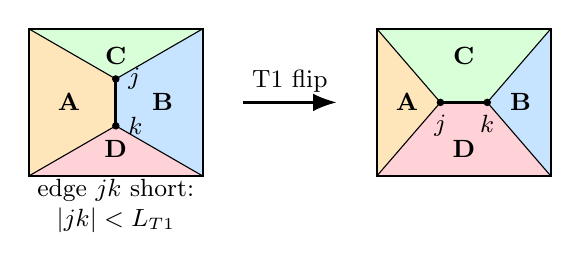
\begin{tikzpicture}[scale=0.85, every node/.style={font=\small}]
  % ---------------- BEFORE ----------------
  \begin{scope}
    \coordinate (j) at (0,0.35);
    \coordinate (k) at (0,-0.35);
    \coordinate (NW) at (-1.3,1.1);
    \coordinate (NE) at (1.3,1.1);
    \coordinate (SW) at (-1.3,-1.1);
    \coordinate (SE) at (1.3,-1.1);
    \fill[cellB, opacity=0.6] (j) -- (NE) -- (SE) -- (k) -- cycle;
    \fill[cellA, opacity=0.6] (j) -- (k) -- (SW) -- (NW) -- cycle;
    \fill[cellC, opacity=0.6] (NW) -- (j) -- (NE) -- cycle;
    \fill[cellD, opacity=0.6] (SW) -- (k) -- (SE) -- cycle;
    \draw[thick] (NW)--(NE)--(SE)--(SW)--cycle;
    \draw[very thick] (j)--(k);
    \draw (j)--(NW) (j)--(NE) (k)--(SW) (k)--(SE);
    \fill (j) circle(1.6pt) node[right=1pt]{$j$};
    \fill (k) circle(1.6pt) node[right=1pt]{$k$};
    \node at (-0.7,0) {\bfseries A};
    \node at (0.7,0) {\bfseries B};
    \node at (0,0.7) {\bfseries C};
    \node at (0,-0.7) {\bfseries D};
    \node[align=center] at (0,-1.55) {edge $jk$ short:\\ $|jk|<L_{T1}$};
  \end{scope}
  \draw[-{Latex[length=3mm]}, thick] (1.9,0) -- (3.3,0) node[midway, above]{T1 flip};
  % ---------------- AFTER ----------------
  \begin{scope}[xshift=5.2cm]
    \coordinate (jp) at (-0.35,0);
    \coordinate (kp) at (0.35,0);
    \coordinate (NW) at (-1.3,1.1);
    \coordinate (NE) at (1.3,1.1);
    \coordinate (SW) at (-1.3,-1.1);
    \coordinate (SE) at (1.3,-1.1);
    \fill[cellC, opacity=0.6] (NW) -- (jp) -- (kp) -- (NE) -- cycle;
    \fill[cellD, opacity=0.6] (SW) -- (jp) -- (kp) -- (SE) -- cycle;
    \fill[cellA, opacity=0.6] (NW) -- (jp) -- (SW) -- cycle;
    \fill[cellB, opacity=0.6] (NE) -- (kp) -- (SE) -- cycle;
    \draw[thick] (NW)--(NE)--(SE)--(SW)--cycle;
    \draw[very thick] (jp)--(kp);
    \draw (jp)--(NW) (jp)--(SW) (kp)--(NE) (kp)--(SE);
    \fill (jp) circle(1.6pt) node[below=1pt]{$j$};
    \fill (kp) circle(1.6pt) node[below=1pt]{$k$};
    \node at (0,0.7) {\bfseries C};
    \node at (0,-0.7) {\bfseries D};
    \node at (-0.85,0) {\bfseries A};
    \node at (0.85,0) {\bfseries B};
  \end{scope}
\end{tikzpicture}
\caption{The T1 neighbour exchange. Before: $A$ and $B$ share the short
edge $jk$; $C$ and $D$ each touch only at one of its endpoints and are
not neighbours of each other. After: the edge has rotated $90^\circ$
-- $C$ and $D$ now share it and become neighbours, while $A$ and $B$
lose the shared edge and stop being neighbours, each shrinking by one
side as $C$ and $D$ each grow by one side.}
\label{fig:T1}
\end{figure}

\textbf{The rewiring, step by step} (matching
\texttt{try\_T1\_edge} in \texttt{T1\_transition.f90}):
\begin{enumerate}
  \item Identify the two cells $A,B$ owning edge $(j,k)$, and the two
  ``outside'' cells $C$ (the third cell at $j$) and $D$ (the third cell
  at $k$).
  \item Safety checks: both $j$ and $k$ must genuinely be trivalent
  (exactly 3 owning cells each -- defensively skipped otherwise), $A$
  and $B$ must have more than 3 sides (a flip would otherwise shrink
  one below the minimum of 3), and $C,D$ must have room for one more
  side each (\texttt{MAX\_SIDES}).
  \item \textbf{Ring surgery}: insert $k$ into $C$'s ring (next to $j$,
  on the side that used to border $B$) and $j$ into $D$'s ring (next to
  $k$, on the side that used to border $A$); then remove $k$ from $A$'s
  ring and $j$ from $B$'s ring. (The ``which side'' logic, matching
  \texttt{find\_insert\_side} in the code, comes from the four cells
  momentarily meeting at one point in cyclic order $(A,C,B,D)$ as the
  edge shrinks to zero -- when it reopens the other way, the two new
  vertices must separate into groups $\{A,C,D\}$ and $\{B,C,D\}$, which
  is exactly what keeps $C$ attached to $A$'s old side and $D$ attached
  to $B$'s old side.)
  \item \textbf{Reposition}: $j$ and $k$ are physically moved apart,
  along the direction perpendicular to the old edge (within the local
  tangent plane of the shell), by $1.5\times$\texttt{L\_T1\_threshold},
  on both the apical and basal shells -- so the newly created edge
  starts out safely open rather than immediately re-triggering the same
  threshold.
\end{enumerate}
Every cell in the simulation is scanned for short edges once per
topology check; a \texttt{touched} flag on each vertex column ensures a
vertex that was just involved in one flip is not immediately
considered for another flip in the same pass (its ring has just
changed, so any cached side-count/neighbour information about it is
now stale).

\subsection{T2: cell removal (extrusion)}
\label{sec:T2}
\textbf{Biology.} Cells are also removed from a tissue -- through
programmed cell death (apoptosis) or mechanical extrusion, a cell can
shrink until it disappears from the sheet entirely, its neighbours
closing the small gap it leaves behind. The standard vertex-model
counterpart of this is the T2 transition.

\textbf{The rule.} A cell only becomes eligible for a T2 once repeated
T1 events have worn it down to exactly 3 sides (the minimum possible
for a proper polygon) \emph{and} its apical area has shrunk below
\texttt{A\_T2\_threshold}. When both hold, the code collapses the
entire triangular cell to a single point: all 3 of its vertex columns
are merged into their mean position (on both apical and basal shells),
one of the three ids is kept as the survivor, and every other cell in
the mesh that referenced either of the two discarded ids has that
reference globally replaced by the survivor. The cell itself is then
marked dead. The net effect on each of the (up to 3) neighbouring
cells is exactly what you would expect: each loses one side, since two
of its corners have just become the same point.

As with T1, it is worth seeing the collapsing cell as a genuine 3D
vertex column before switching to the flat top-down view used below:

\begin{figure}[h]
\centering
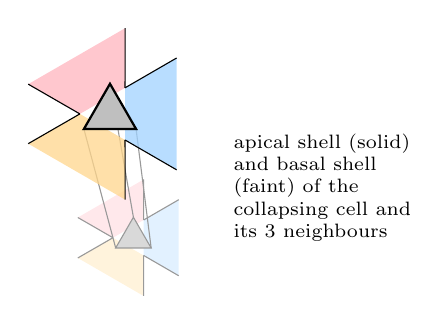
\begin{tikzpicture}[scale=0.85, every node/.style={font=\small}]
  % basal shell (faint): the identical construction, scaled down and
  % shifted, exactly the pseudo-3D convention of Fig.~\ref{fig:one-cell}
  \begin{scope}[shift={(0.35,-1.85)}, scale=0.68]
    \foreach \ang/\col in {90/cellA, 210/cellB, 330/cellD} {
      \begin{scope}[rotate=\ang]
        \fill[\col, opacity=0.3] (90:0.45) -- (110:1.3) -- (190:1.3) -- (210:0.45) -- cycle;
        \draw[black!40] (90:0.45) -- (110:1.3) (210:0.45) -- (190:1.3);
      \end{scope}
    }
    \draw[black!40, fill=black!15] (90:0.45) -- (210:0.45) -- (330:0.45) -- cycle;
  \end{scope}
  % lateral walls (struts) from the collapsing triangle's own 3
  % corners down to their basal echo
  \foreach \ang in {90,210,330} {
    \draw[thin, black!40] (\ang:0.45) -- ($(0.35,-1.85)+0.68*(\ang:0.45)$);
  }
  % apical shell (solid), on top -- the collapsing cell and its 3
  % neighbours, as genuine 3D vertex columns
  \foreach \ang/\col in {90/cellA, 210/cellB, 330/cellD} {
    \begin{scope}[rotate=\ang]
      \fill[\col, opacity=0.75] (90:0.45) -- (110:1.3) -- (190:1.3) -- (210:0.45) -- cycle;
      \draw (90:0.45) -- (110:1.3) (210:0.45) -- (190:1.3);
    \end{scope}
  }
  \draw[thick, fill=black!25] (90:0.45) -- (210:0.45) -- (330:0.45) -- cycle;
  \node[right, font=\scriptsize, align=left] at (1.7,-1.1) {apical shell (solid)\\and basal shell\\(faint) of the\\collapsing cell and\\its 3 neighbours};
\end{tikzpicture}
\caption{The collapsing triangular cell and its 3 neighbours, drawn as
genuine 3D vertex columns: solid = apical shell, faint = basal shell
(shifted for the pseudo-3D view of Fig.~\ref{fig:one-cell}). The T2
collapse below happens to both shells at once -- every merged vertex
column has its apical \emph{and} basal point averaged together, exactly
as \texttt{collapse\_cell} does in the code (Section~\ref{sec:T2}).}
\label{fig:T2-3d}
\end{figure}

Fig.~\ref{fig:T2-3d} is, again, easiest to reason about from directly
above -- the same top-down (apical) view used for T1:

\begin{figure}[h]
\centering
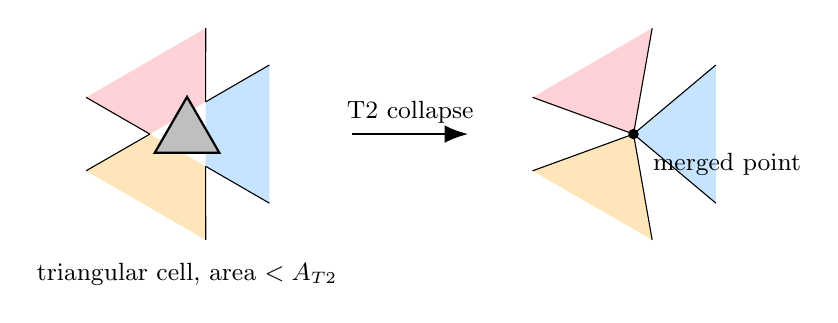
\begin{tikzpicture}[scale=1.05, every node/.style={font=\small}]
  \begin{scope}
    \foreach \ang/\col in {90/cellA, 210/cellB, 330/cellD} {
      \begin{scope}[rotate=\ang]
        \fill[\col, opacity=0.6] (90:0.45) -- (110:1.3) -- (190:1.3) -- (210:0.45) -- cycle;
        \draw (90:0.45) -- (110:1.3) (210:0.45) -- (190:1.3);
      \end{scope}
    }
    \draw[thick, fill=black!25] (90:0.45) -- (210:0.45) -- (330:0.45) -- cycle;
    \node[align=center] at (0,-1.7) {triangular cell, area $< A_{T2}$};
  \end{scope}
  \draw[-{Latex[length=3mm]}, thick] (2.0,0) -- (3.4,0) node[midway, above]{T2 collapse};
  \begin{scope}[xshift=5.4cm]
    \foreach \ang/\col in {90/cellA, 210/cellB, 330/cellD} {
      \begin{scope}[rotate=\ang]
        \fill[\col, opacity=0.6] (0,0) -- (110:1.3) -- (190:1.3) -- cycle;
        \draw (0,0) -- (110:1.3) (0,0) -- (190:1.3);
      \end{scope}
    }
    \fill (0,0) circle (1.8pt) node[below right=5pt] {merged point};
  \end{scope}
\end{tikzpicture}
\caption{The T2 transition. A 3-sided cell whose area has fallen below
\texttt{A\_T2\_threshold} collapses to a single merged vertex; each of
its (up to 3) neighbours loses exactly one side.}
\label{fig:T2}
\end{figure}

\textbf{Cascades.} Occasionally this collapse itself pushes a
\emph{neighbouring} cell below 3 sides -- e.g. two T2-eligible triangles
sharing an edge. Rather than leave a degenerate cell behind,
\texttt{do\_T2} keeps a small bounded queue (\texttt{QCAP} slots): any
neighbour pushed below 3 sides by a collapse is queued and forcibly
collapsed the same way, which may itself queue further neighbours. The
queue is drained until nothing more needs collapsing -- bounded so that
even a pathological mesh cannot loop forever.

\subsection{Cell division}
\label{sec:division}
\textbf{Biology.} Tissues also grow: cells accumulate volume and
eventually divide (mitosis) into two daughters. Here a cell becomes
eligible once its volume exceeds
\texttt{V\_division\_threshold}$\,\times V_i^0$ (checked only if
\texttt{division\_enable} is on).

\textbf{The division axis.} A random ring index $k_1$ is chosen, and
its ``roughly opposite'' edge $k_2 = k_1 + \lfloor n/2\rfloor$ (wrapped
around the ring) -- for a hexagon, literally the opposite edge; for an
odd-sided polygon, the closest edge to opposite. New vertex columns
are inserted at the midpoint of each of these two edges, on
\emph{both} the apical and basal shells, and the parent's ring is cut
into two contiguous arcs at those two new vertices -- each arc, closed
off by the new shared edge between the two new vertices, becomes one
daughter cell.

Once again, it helps to see this happening to a genuine 3D vertex
column, cut all the way from its apical face down to its basal face,
before looking at the flat top-down view used for the rest of this
section:

\begin{figure}[h]
\centering
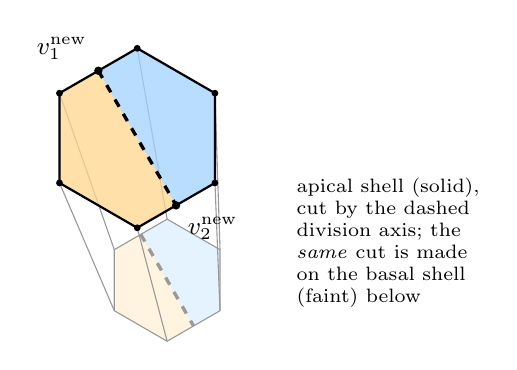
\begin{tikzpicture}[scale=0.95, every node/.style={font=\small}]
  \foreach \i in {1,...,6}{
    \coordinate (P\i) at ({90+60*(\i-1)}:1.2);
  }
  \coordinate (V1) at ($(P1)!0.5!(P2)$);
  \coordinate (V2) at ($(P4)!0.5!(P5)$);
  % basal shell (faint): same hexagon and same cut, scaled down and
  % shifted, exactly the pseudo-3D convention of Fig.~\ref{fig:one-cell}
  \begin{scope}[shift={(0.4,-1.9)}, scale=0.68]
    \coordinate (P1B) at (90:1.2); \coordinate (P2B) at (150:1.2);
    \coordinate (P3B) at (210:1.2); \coordinate (P4B) at (270:1.2);
    \coordinate (P5B) at (330:1.2); \coordinate (P6B) at (30:1.2);
    \coordinate (V1B) at ($(P1B)!0.5!(P2B)$);
    \coordinate (V2B) at ($(P4B)!0.5!(P5B)$);
    \fill[cellA, opacity=0.28] (V1B) -- (P2B) -- (P3B) -- (P4B) -- (V2B) -- cycle;
    \fill[cellB, opacity=0.28] (V2B) -- (P5B) -- (P6B) -- (P1B) -- (V1B) -- cycle;
    \draw[black!40] (P1B)--(P2B)--(P3B)--(P4B)--(P5B)--(P6B)--cycle;
    \draw[very thick, dashed, black!40] (V1B) -- (V2B);
  \end{scope}
  % lateral walls (struts)
  \foreach \i in {1,...,6}{
    \draw[thin, black!40] (P\i) -- ($(0.4,-1.9)+0.68*(P\i)$);
  }
  % apical shell (solid) -- identical to the panel of Fig.~\ref{fig:division} below
  \fill[cellA, opacity=0.75] (V1) -- (P2) -- (P3) -- (P4) -- (V2) -- cycle;
  \fill[cellB, opacity=0.75] (V2) -- (P5) -- (P6) -- (P1) -- (V1) -- cycle;
  \draw[thick] (P1)--(P2)--(P3)--(P4)--(P5)--(P6)--cycle;
  \draw[very thick, dashed] (V1) -- (V2);
  \foreach \p in {P1,P2,P3,P4,P5,P6} { \fill (\p) circle (1.3pt); }
  \fill (V1) circle (1.6pt) node[above left=1pt] {$v_1^{\mathrm{new}}$};
  \fill (V2) circle (1.6pt) node[below right=1pt] {$v_2^{\mathrm{new}}$};
  \node[right, font=\scriptsize, align=left] at (2.0,-1.4) {apical shell (solid),\\cut by the dashed\\division axis; the\\\emph{same} cut is made\\on the basal shell\\(faint) below};
\end{tikzpicture}
\caption{The dividing cell as a genuine 3D vertex column: solid =
apical shell, faint = basal shell (shifted for the pseudo-3D view of
Fig.~\ref{fig:one-cell}). The dashed division axis is cut on
\emph{both} shells -- \texttt{do\_division} inserts a new vertex column
(with its own apical \emph{and} basal position) at each bisected edge,
exactly as for $v_1^{\mathrm{new}}, v_2^{\mathrm{new}}$ here.}
\label{fig:division-3d}
\end{figure}

Flattened to the top-down (apical) view used for the rest of this
section, the same division looks like this:

\begin{figure}[h]
\centering
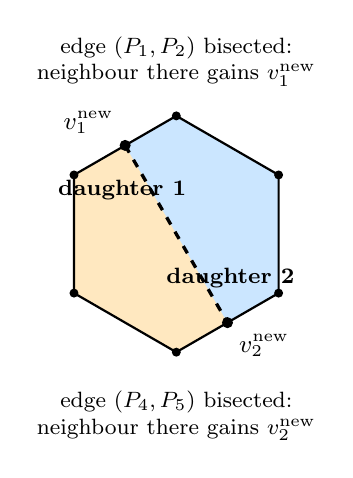
\begin{tikzpicture}[scale=1.25, every node/.style={font=\small}]
  \coordinate (P1) at (90:1.2);
  \coordinate (P2) at (150:1.2);
  \coordinate (P3) at (210:1.2);
  \coordinate (P4) at (270:1.2);
  \coordinate (P5) at (330:1.2);
  \coordinate (P6) at (30:1.2);
  \coordinate (V1) at ($(P1)!0.5!(P2)$);
  \coordinate (V2) at ($(P4)!0.5!(P5)$);
  \fill[cellA, opacity=0.55] (V1) -- (P2) -- (P3) -- (P4) -- (V2) -- cycle;
  \fill[cellB, opacity=0.55] (V2) -- (P5) -- (P6) -- (P1) -- (V1) -- cycle;
  \draw[thick] (P1)--(P2)--(P3)--(P4)--(P5)--(P6)--cycle;
  \draw[very thick, dashed] (V1) -- (V2);
  \foreach \p in {P1,P2,P3,P4,P5,P6} { \fill (\p) circle (1.3pt); }
  \fill (V1) circle (1.6pt) node[above left=1pt] {$v_1^{\mathrm{new}}$};
  \fill (V2) circle (1.6pt) node[below right=1pt] {$v_2^{\mathrm{new}}$};
  \node[font=\footnotesize\bfseries] at (-0.55,0.45) {daughter 1};
  \node[font=\footnotesize\bfseries] at (0.55,-0.45) {daughter 2};
  \node[align=center, font=\footnotesize] at (0,1.75) {edge $(P_1,P_2)$ bisected:\\ neighbour there gains $v_1^{\mathrm{new}}$};
  \node[align=center, font=\footnotesize] at (0,-1.85) {edge $(P_4,P_5)$ bisected:\\ neighbour there gains $v_2^{\mathrm{new}}$};
\end{tikzpicture}
\caption{Cell division. Two roughly-opposite edges are bisected with
new vertex columns $v_1^{\mathrm{new}}, v_2^{\mathrm{new}}$ (inserted on
both apical and basal shells); the parent's ring splits into two arcs
along the new dashed shared edge, each arc becoming one daughter cell.
The two neighbouring cells whose edges were bisected each gain one new
side, since their ring now also includes the corresponding new vertex.}
\label{fig:division}
\end{figure}

\textbf{Bookkeeping.} Both daughters inherit half of the parent's
target volume and area, $V^0_{\text{daughter}} = \tfrac12 V^0_{\text{parent}}$,
$A^0_{\text{daughter}} = \tfrac12 A^0_{\text{parent}}$ -- so immediately
after dividing, neither daughter starts under artificial elastic
stress from suddenly being half the size of its own target. The (at
most two) neighbouring cells whose edges were bisected are spliced to
include the corresponding new vertex, gaining one side each. As with
T1 and T2, \texttt{do\_division} validates everything first --
polygon-size limits (\texttt{len1,len2} both between 3 and
\texttt{MAX\_SIDES}), vertex/cell array capacity, and every affected
neighbour's side-count headroom (including the edge case where the
\emph{same} third cell happens to border the parent along both cut
edges, needing room for \emph{two} new sides, not one) -- and only
allocates the two new vertex columns and the new cell slot once every
check has passed.

\section{Sanity checks and worked benchmarks}
\label{sec:code-sanity}

\subsection{A worked check: turning on the basal terms}
\label{sec:basal-benchmark}
Section~\ref{sec:energy} introduced $K_A^{\mathrm{bas}}, K_P^{\mathrm{bas}},
A^{0,\mathrm{bas}}$ as independent basal-face moduli/target, defaulting
to their apical counterparts if left unset. Before trusting that code
at all, it was checked the same way every other geometric quantity in
this project is checked (Section~\ref{sec:mod-sanity}): the unit-cube
self-test (\texttt{test\_cube\_volume}) was extended to also assert
$A^{\mathrm{bas}}=1$ for the cube's basal (unit-square) face, which it
does, exactly, at start-up, on every run. With that primitive-level
check passing, three full runs (same geodesic mesh, $L=2$, 162 cells;
same $\Lambda=+0.1$ so the tissue relaxes smoothly rather than hitting
the instability of Section~\ref{sec:instability} below; $10^5$ steps
each) were compared, differing only in the basal moduli:
\begin{center}
\begin{tabular}{@{}lccc@{}}
\toprule
 & \textbf{zero basal} & \textbf{equal to apical} & \textbf{different} \\
$K_A^{\mathrm{bas}}$ & $0$ & $1.0$ (=$K_A$) & $5.0$ \\
$K_P^{\mathrm{bas}}$ & $0$ & $0.05$ (=$K_P$) & $0.5$ \\
$A^{0,\mathrm{bas}}$ scale & -- & $1.0\times$ initial & $1.2\times$ initial \\
\midrule
$E(t{=}0)$                 & $6298.1$ & $10580.4$ & $29672.2$ \\
$E(t{=}\mathrm{end})$      & $464.6$  & $845.8$   & $5020.9$ \\
final $\max|\vec F|$       & $3.0\times10^{-3}$ & $3.2\times10^{-5}$ & $1.1\times10^{-12}$ \\
final mean $A^{\mathrm{bas}}$ & $6.73$ & $6.58$ & $7.45$ \\
\bottomrule
\end{tabular}
\end{center}
All three runs stayed perfectly well behaved throughout: the
lumen volume (Section~\ref{sec:basal-reverse}) stayed positive the
whole time, no NaNs appeared anywhere, the Euler-characteristic and
ring-integrity checks passed at every check, and no T1/T2 events were
needed (a smooth, symmetric relaxation from an already-close-to-round
starting mesh). A few things are worth reading off this table
directly:
\begin{itemize}[leftmargin=1.4em]
  \item \textbf{Zero basal moduli reproduces the old, apical-only
  behaviour exactly}, as it must: with $K_A^{\mathrm{bas}}=K_P^{\mathrm{bas}}=0$,
  every new term in Eq.~\ref{eq:energy} and every new contribution to
  Eq.~\ref{eq:dE-bas} is multiplied by zero, so the physics is
  bit-for-bit what it would be without this feature at all -- this is
  the natural regression benchmark for the change, and it holds by
  construction, not just in this one run.
  \item \textbf{Turning on matching basal terms makes the tissue settle
  \emph{more precisely}} into its equilibrium: the final residual
  force drops by almost two orders of magnitude (from $3\times10^{-3}$
  to $3\times10^{-5}$) simply because the basal face now has its own
  restoring forces pulling it towards a well-defined equilibrium shape,
  on top of what volume and lateral tension already provided.
  \item \textbf{Giving the basal face a genuinely different target}
  (here, $20\%$ larger than its initial area, with a stiffer modulus
  to go with it) drives the tissue to a \emph{different, still stable}
  equilibrium: the basal face grows towards its enlarged target ($6.92
  \to 7.45$, on the way to $8.30$ -- not all the way, since the other
  terms resist the pull), and -- because every cell's apical, basal and
  lateral faces are mechanically coupled through the shared volume and
  lateral-tension terms -- the apical face and the lumen volume both
  expand too, even though nothing was changed about the apical
  parameters directly. The residual force here is smaller still
  ($10^{-12}$, essentially machine precision): a real energy minimum
  was found, not a numerical artefact, and it was found in the
  \emph{correct direction} (growing, as the enlarged target demands,
  rather than shrinking or diverging) -- good evidence that the sign
  of the new force terms in Eq.~\ref{eq:dE-bas} is correct.
\end{itemize}
This is exactly the kind of asymmetric apical--basal behaviour the
independent moduli make possible: a tissue whose basal side is, say,
attached to a stiffer real basement membrane can now be modelled by
simply giving it a larger $K_A^{\mathrm{bas}}$, without touching
anything on the apical side.

\subsection{A known instability: strongly negative lateral tension}
\label{sec:instability}
One physics result worth flagging explicitly, because it comes
straight out of the model (Eq.~\ref{eq:energy}) and is not a coding
bug: nothing in this energy functional stops a cell from
geometrically passing through its neighbours. A \emph{positive}
$\Lambda$ (lateral tension resists stretching the cell--cell contact,
Section~\ref{sec:energy}) keeps the tissue well behaved -- in practice
the largest force over all vertices (\texttt{max\_force} in the
diagnostics, Section~\ref{sec:io-module-code}) decays towards zero as
the tissue relaxes to a mechanical equilibrium. A strongly
\emph{negative} $\Lambda$, by contrast, acts as a \emph{negative}
surface tension: it actively rewards \emph{growing} the contact area
between neighbours, with nothing in Eq.~\ref{eq:energy} to stop that
growth once cells start overlapping rather than merely touching. In
practice this shows up first as a checkerboard-like buckling pattern
across the tissue, then as an outright geometric collapse -- cells
sliding over one another while the topology (Section
\ref{sec:transitions}) can remain perfectly self-consistent throughout
(the Euler-characteristic and ring-integrity checks of
Section~\ref{sec:mod-sanity} are purely \emph{combinatorial}: they
confirm the mesh's connectivity makes sense, not that its embedding in
3D space is still non-self-intersecting). The one diagnostic that
\emph{does} catch this unambiguously is the lumen volume
(Section~\ref{sec:basal-reverse}): a closed surface's enclosed volume
can only come out negative if that surface has folded over itself,
which is exactly what \texttt{write\_diagnostics\_now}
(Section~\ref{sec:main-code}) checks for, printing an explicit runtime
warning the moment it happens. This is a genuine limitation of the
standard vertex-model energy itself (shared by essentially every
model of this family), not merely of this particular implementation --
a hard non-overlap constraint would need to be added separately if it
mattered for a given application.

\chapter{Code implementation}
\label{ch:code}

Chapter~\ref{ch:theory} explained \emph{what} is being computed and
\emph{why}. This chapter explains \emph{where}, in the actual source
code, every one of those pieces lives, in enough detail that you could
find and modify any specific behaviour. It walks through every single
subroutine and function in the project, in the order they naturally
build on each other, always giving the \textbf{physical meaning first,
with the code's own variable or routine name in parentheses}, e.g.
``the apical position (\texttt{r\_api}) of vertex column $j$''. The
Fortran engine (Section~\ref{sec:src-code}) does all the physics; the
MATLAB scripts (Section~\ref{sec:matlab-code}) read its binary output
and turn it into pictures.

\section{Directory map}
\label{sec:dirmap}
\begin{figure}[h]
\centering
\begin{forest}
for tree={
  font=\ttfamily,
  grow'=0,
  edge={gray},
  parent anchor=south west,
  child anchor=west,
  anchor=west,
  s sep=5pt,
}
[{Vertex\_Model\_3d/}
  [{README.md}]
  [{para.in}]
  [{Makefile}]
  [{src/ \textrm{\normalfont\itshape\small\ -- 14 files, the Fortran engine, Sec.~\ref{sec:src-code}}}]
  [{build/}]
  [{data/ \textrm{\normalfont\itshape\small\ -- snap\_/diag\_ output + example/}}]
  [{matlab/ \textrm{\normalfont\itshape\small\ -- 14 files, analysis \& plotting, Sec.~\ref{sec:matlab-code}}}]
  [{videos/}]
  [{docs/}]
]
\end{forest}
\caption{Top level of the project. \texttt{src/} and \texttt{matlab/}
each contain many files, listed in full (with the section that
explains them) just below; \texttt{build/}, \texttt{data/} (except
\texttt{data/example/}) and \texttt{videos/} are generated
automatically and are not stored in version control.}
\label{fig:dirmap}
\end{figure}

\begin{center}
\begin{minipage}{0.46\textwidth}
\centering \textbf{src/} (Section~\ref{sec:src-code})\vspace{2pt}\\
{\ttfamily\small\begin{tabular}{@{}l@{}}
mod\_kinds.f90\\ mod\_parameters.f90\\ mod\_data.f90\\
mod\_geometry.f90\\ mod\_topology.f90\\ mesh\_init.f90\\
Force.f90\\ Langevin\_update.f90\\ T1\_transition.f90\\
T2\_transition.f90\\ Cell\_Division.f90\\ io\_module.f90\\
sanity\_checks.f90\\ main.f90
\end{tabular}}
\end{minipage}%
\begin{minipage}{0.5\textwidth}
\centering \textbf{matlab/} (Section~\ref{sec:matlab-code})\vspace{2pt}\\
{\ttfamily\small\begin{tabular}{@{}l@{}}
main\_analysis.m \ \ main\_movie.m\\
read\_vertex\_snapshot.m \ \ read\_diagnostics.m\\
read\_mesh\_meta.m\\
list\_snapshots.m \ \ list\_diagnostics.m\\
select\_snapshots.m\\
cell\_faces\_matrix.m \ \ tissue\_color\_values.m\\
plot\_tissue\_3d.m \ \ plot\_cross\_section.m\\
make\_tissue\_video.m\\
make\_cross\_section\_video.m
\end{tabular}}
\end{minipage}
\end{center}

\section{The Fortran engine (\texttt{src/})}
\label{sec:src-code}
The 14 source files are compiled in a strict dependency order (each
Fortran \texttt{module} must be compiled before anything that
\texttt{use}s it) -- this order is also, conveniently, close to the
most natural \emph{reading} order, going from the most low-level/generic
building blocks up to the program that ties everything together:
\texttt{mod\_kinds} $\rightarrow$ \texttt{mod\_parameters} $\rightarrow$
\texttt{mod\_data} $\rightarrow$ \texttt{mod\_geometry} $\rightarrow$
\texttt{mod\_topology} $\rightarrow$ \texttt{mesh\_init} $\rightarrow$
\texttt{Force} $\rightarrow$ \texttt{Langevin\_update} $\rightarrow$
\texttt{T1\_transition} $\rightarrow$ \texttt{T2\_transition}
$\rightarrow$ \texttt{Cell\_Division} $\rightarrow$ \texttt{io\_module}
$\rightarrow$ \texttt{sanity\_checks} $\rightarrow$ \texttt{main}.

\subsection{\texttt{mod\_kinds.f90} -- numeric precision}
The entire codebase works in one consistent numeric precision, defined
here once and \texttt{use}d by literally every other module:
\texttt{dp} (\emph{double precision}, an 8-byte floating-point number
-- every physical quantity: positions, forces, energies, parameters)
and \texttt{i4} (a 4-byte integer -- every count: vertex ids, cell ids,
loop indices). Centralising these avoids ever mixing precisions by
accident. This file defines no subroutines, only these two named
constants.

\subsection{\texttt{mod\_parameters.f90} -- the parameter file reader}
\paragraph{Reads the simulation parameters (\texttt{read\_parameters}).}
\textbf{Input:} a file name (\texttt{fname}, in practice always
\texttt{"para.in"}). \textbf{Output:} none as a return value -- instead
it fills in roughly two dozen \texttt{module}-level variables (visible
to every other module that \texttt{use}s \texttt{mod\_parameters}),
covering every physical modulus in Chapter~\ref{ch:theory}
($K_V,K_A,K_P,\Lambda$ as \texttt{K\_V,K\_A,K\_P,Lambda\_line}, and
their basal counterparts $K_A^{\mathrm{bas}}, K_P^{\mathrm{bas}}$ as
\texttt{K\_A\_bas, K\_P\_bas}), every geometric/mesh setting
(\texttt{N\_subdivision, R\_apical, R\_basal}), every dynamics setting
(\texttt{zeta\_friction, kBT, dt, n\_steps}), and every transition
threshold (\texttt{L\_T1\_threshold, A\_T2\_threshold,
V\_division\_threshold}, and how often to check for each).
\textbf{Calls:} only Fortran intrinsics (it reads a \texttt{NAMELIST}
block, Fortran's native ``named key=value list'' file format). It also
runs a handful of basic sanity checks on the values themselves (e.g.
$R_{\mathrm{basal}}>0$ and $R_{\mathrm{apical}}>R_{\mathrm{basal}}$,
$dt>0$) and stops the program immediately with a clear message if any
of them look nonsensical, rather than silently running a broken
simulation. One subtlety here: \texttt{K\_A\_bas}, \texttt{K\_P\_bas}
and \texttt{A0\_bas\_scale} (the basal-face target-area scale,
Section~\ref{sec:energy}) are given a negative sentinel default
(\texttt{-1.0}) \emph{before} the file is read; if \texttt{para.in}
does not set them explicitly they are left negative by the read, and a
short fix-up right after it replaces each still-negative one with its
apical counterpart (\texttt{K\_A}, \texttt{K\_P}, \texttt{A0\_scale}).
This is exactly the same trick already used for
\texttt{capacity\_growth\_factor} (a fixed default, rather than a
sentinel, since it doesn't need to mirror another variable) -- it lets
an older \texttt{para.in} with no basal keys at all keep working
unchanged, with the basal face defaulting to behave exactly like the
apical one.

\subsection{\texttt{mod\_data.f90} -- the core data structures}
This file defines the two central data structures literally everything
else in the code operates on.

\paragraph{A cell (\texttt{cell\_t}).} A Fortran derived type
representing one cell as a polygon ring: how many sides it currently
has (\texttt{n}), the ordered list of vertex-column ids going around it
(\texttt{vlist}, padded with zeros up to \texttt{MAX\_SIDES}=16, the
hard cap on polygon valence), whether the slot is currently in use
(\texttt{alive} -- cells removed by a T2 event are marked
\texttt{.false.} rather than physically deleted from the array, so
other cells' stored ids into the array stay valid), and its target
volume/apical-area/basal-area and most-recently-computed
volume/apical-area/basal-area
($V^0,A^0,A^{0,\mathrm{bas}},V,A_{\mathrm{api}},A_{\mathrm{bas}}$ as
\texttt{V0, A0, A0\_bas, V\_last, A\_last, A\_bas\_last}).

\paragraph{The global vertex/cell arrays.} Every vertex column's apical
and basal positions ($\rvec_{\mathrm{api}}, \rvec_{\mathrm{bas}}$ as
\texttt{r\_api(:,j), r\_bas(:,j)}, each a $3\times$\texttt{n\_vert\_cap}
array) and forces ($\fapi{j},\fbas{j}$ as \texttt{f\_api, f\_bas}), a
per-slot alive flag (\texttt{vert\_alive}), and the whole array of
cells (\texttt{cells(:)}, of type \texttt{cell\_t}). All of these are
\texttt{allocatable} rather than fixed-size, since the cell/vertex
count changes as the simulation runs (division creates new ones; T2
removes some).

\paragraph{Allocates/resets all of the above (\texttt{allocate\_data}).}
\textbf{Inputs:} the number of cells and vertex columns needed right
now (\texttt{ncell\_init, nvert\_init}), and an optional
\emph{headroom} multiplier (\texttt{growth\_factor}, default
$2\times$; the actual run uses \texttt{capacity\_growth\_factor} from
\texttt{para.in}). \textbf{Output:} none directly -- it
(re-)\texttt{allocate}s every global array above, sized to
$\max(\text{count}, \text{count}\times\text{growth\_factor})$ so that
cell division has somewhere to put new cells/vertices without needing
to resize (Fortran arrays cannot cheaply grow in place) mid-run, and
zeroes/resets everything. \textbf{Calls:} none (pure Fortran
\texttt{allocate} statements). Called once by \texttt{init\_mesh} to
size things for the very first mesh, and once (with a tiny,
throw-away size) by each of the two start-up self-tests in
\texttt{sanity\_checks.f90}, before being re-called (safely) at the
real size.

\paragraph{Counts living cells/vertices (\texttt{count\_alive\_cells},
\texttt{count\_alive\_verts}).} \textbf{Input:} none (they read the
global \texttt{cells}/\texttt{vert\_alive} arrays directly).
\textbf{Output:} an integer count. \textbf{Calls:} none. Simple loops
used everywhere a current cell/vertex count is needed (progress
messages, diagnostics, capacity checks).

\subsection{\texttt{mod\_geometry.f90} -- geometric primitives}
The exact building blocks derived in full in
Sections~\ref{sec:tetra-vol}--\ref{sec:tri-area}: this file has no
knowledge of cells or the tissue at all, only bare vectors.
\paragraph{Cross product (\texttt{cross}) and length (\texttt{norm3}).}
Ordinary vector algebra helpers, $\vec a\times\vec b$ and $|\vec a|$,
used throughout the rest of the codebase.
\paragraph{Tetrahedron volume and its gradient (\texttt{tetra\_vol\_grad}).}
\textbf{Inputs:} three points \texttt{p, q, r}. \textbf{Outputs:} the
signed volume \texttt{vol} (Eq.~\ref{eq:tetra-vol}) and its three exact
gradients \texttt{gp, gq, gr} (Eq.~\ref{eq:tetra-grad}).
\textbf{Calls:} \texttt{cross}. This is the single most-called routine
in the whole physics engine (it runs once for every fan triangle of
every cell's apical cap, basal cap, and lateral walls, every single
time step).
\paragraph{Triangle area and its gradient (\texttt{tri\_area\_grad}).}
\textbf{Inputs:} three points \texttt{p, q, r}. \textbf{Outputs:} the
area \texttt{area} and its three exact gradients \texttt{gp, gq, gr}
(Eq.~\ref{eq:tri-grad}), plus optionally the unit normal
\texttt{nhat\_out}. \textbf{Calls:} \texttt{cross}, \texttt{norm3}.
\paragraph{Centroid of $n$ points (\texttt{centroid\_n}).}
\textbf{Inputs:} an array of $n$ points \texttt{pts} and the count
\texttt{n}. \textbf{Output:} their plain average (Section~\ref{sec:fan}'s
$\ca$ or $\cb$). \textbf{Calls:} none. Used once per cell for the
apical centroid and once for the basal centroid, in
\texttt{compute\_forces}.

\subsection{\texttt{mod\_topology.f90} -- ring surgery toolkit}
\label{sec:mod-topology}
This file has no knowledge of \emph{physics} at all -- purely
combinatorial operations on the ring data structure
(\texttt{cells(:)\%vlist}), kept deliberately independent of
\texttt{mod\_geometry} (a design choice noted in the file's own header
comment). T1, T2 and cell division are all built out of these same
handful of primitives.
\paragraph{Find a vertex's position in a ring (\texttt{ring\_find}).}
\textbf{Inputs:} a cell id \texttt{icell} and a vertex-column id
\texttt{vid}. \textbf{Output:} its 1-based slot number in that cell's
\texttt{vlist} (0 if not present). \textbf{Calls:} none. The single
most-used lookup in this file.
\paragraph{Check whether two vertices are ring-adjacent
(\texttt{ring\_has\_edge}).} \textbf{Inputs:} \texttt{icell, v1, v2}.
\textbf{Output:} true if \texttt{v1,v2} are consecutive (in either
order) in that cell's ring, i.e. genuinely share an edge of that cell.
\textbf{Calls:} none.
\paragraph{Find the (up to 2) cells owning an edge (\texttt{edge\_cells}).}
\textbf{Inputs:} two vertex-column ids \texttt{v1, v2}.
\textbf{Outputs:} the (up to two) alive cell ids \texttt{cA, cB} whose
ring contains that edge (0 if fewer than two are found -- on a proper
closed mesh every edge belongs to exactly two cells, so a 0 here is a
red flag). \textbf{Calls:} \texttt{ring\_has\_edge}, once per alive
cell (a linear scan -- simple and, for the cell counts this code
targets, fast enough).
\paragraph{Find every cell touching a vertex (\texttt{vertex\_incidence}).}
\textbf{Input:} a vertex-column id \texttt{vid}. \textbf{Outputs:} the
list of alive cell ids containing it (\texttt{list}) and how many
(\texttt{count} -- normally exactly 3, the trivalent rule of
Section~\ref{sec:T1}). \textbf{Calls:} \texttt{ring\_find}, once per
alive cell.
\paragraph{Remove a vertex from a ring (\texttt{ring\_remove}).}
\textbf{Inputs:} \texttt{icell, vid}. \textbf{Output:} success flag
\texttt{ok} (also false if the resulting ring would have fewer than 3
sides). \textbf{Calls:} \texttt{ring\_find}. Shifts every later entry
in \texttt{vlist} down by one slot.
\paragraph{Insert a vertex into a ring (\texttt{ring\_insert\_after}).}
\textbf{Inputs:} \texttt{icell}, an existing vertex id to insert after
(\texttt{after\_vid}), and the new vertex id (\texttt{new\_vid}).
\textbf{Output:} success flag \texttt{ok} (false if \texttt{after\_vid}
is not found, or if the ring is already at \texttt{MAX\_SIDES}).
\textbf{Calls:} \texttt{ring\_find}. Shifts later entries up by one
slot to make room.
\paragraph{Globally substitute one vertex id for another
(\texttt{ring\_replace}).} \textbf{Inputs:} \texttt{icell, old\_vid,
new\_vid}. \textbf{Output:} none (mutates \texttt{cells(icell)\%vlist}
in place, same length). \textbf{Calls:} none. This is the core move
behind a T2 event's vertex merge (Section~\ref{sec:T2}): called once
per remaining alive cell to replace every reference to a discarded
vertex id.
\paragraph{Collapse duplicate ring entries (\texttt{collapse\_duplicates}).}
\textbf{Input:} \texttt{icell}. \textbf{Output:} none (shortens
\texttt{vlist} in place if any two cyclically-consecutive entries are
now equal, which \texttt{ring\_replace} can create when two of a
cell's corners get merged onto the same surviving vertex). \textbf{Calls:}
none. Always used immediately after \texttt{ring\_replace} during a T2
event.
\paragraph{Insert a vertex between two known-adjacent ones
(\texttt{insert\_between}).} \textbf{Inputs:} \texttt{icell}, two
already-adjacent vertex ids \texttt{va, vb} (in \emph{either} order --
two cells sharing an edge walk their own rings in opposite directions,
so this cannot assume which order a given cell sees them in), and the
new vertex \texttt{newv}. \textbf{Output:} success flag \texttt{ok}.
\textbf{Calls:} \texttt{ring\_find}, \texttt{ring\_insert\_after}. Used
by cell division to splice a new mid-edge vertex into a bisected
neighbour's ring.
\paragraph{Allocate a free cell/vertex slot (\texttt{next\_free\_cell\_slot},
\texttt{next\_free\_vert\_slot}).} \textbf{Input:} none.
\textbf{Output:} a slot id (0 if none available, i.e. capacity
exhausted). \textbf{Calls:} none. Both mark the returned slot
``alive'' \emph{immediately}, before returning, specifically so that
two back-to-back calls (e.g. cell division needs two new vertex
columns at once) can never be handed the same free slot twice; the
caller is still responsible for filling in the slot's real position/
ring/target values afterwards.
\paragraph{Euler-characteristic check (\texttt{euler\_check}).}
\textbf{Input:} none (reads global state). \textbf{Outputs:} pass/fail
flag \texttt{ok}, and the raw counts \texttt{V} (alive vertex columns),
\texttt{E} (alive edges, $=\tfrac12\sum_{\text{cells}} n$, since every
edge is shared by exactly two cells), \texttt{F} (alive cells), and the
Euler characteristic \texttt{chi}$=V-E+F$, which must equal exactly 2
for any closed, genus-0 (sphere-like, no holes) surface -- the
fundamental topological invariant this whole mesh must always satisfy,
checked after every batch of T1/T2/division events (via
\texttt{topology\_check} in \texttt{sanity\_checks.f90}, Section
\ref{sec:mod-sanity}). \textbf{Calls:} \texttt{count\_alive\_verts}.

\subsection{\texttt{mesh\_init.f90} -- building the starting tissue}
\label{sec:mesh-init-code}
This file builds everything described in
Section~\ref{sec:mesh-build}: a geodesic icosahedral sphere, then its
dual tessellation.
\paragraph{Builds the whole initial mesh (\texttt{init\_mesh}).}
\textbf{Input:} none directly (reads \texttt{N\_subdivision, R\_apical,
R\_basal} from \texttt{mod\_parameters}). \textbf{Output:} none as a
return value -- it fills in every global array in
\texttt{mod\_data} (\texttt{cells(:), r\_api, r\_bas, vert\_alive}) for
the very first, unstrained tissue. \textbf{Calls, in order:}
\texttt{build\_icosahedron}, \texttt{subdivide\_once} ($L=$
\texttt{N\_subdivision} times), \texttt{fix\_face\_orientation},
\texttt{allocate\_data}, \texttt{dual\_vertex\_position} (once per
triangle face), \texttt{build\_cell\_ring} (once per original
icosahedron/subdivided-sphere vertex), and finally
\texttt{sanity\_check\_degrees}. This is the only place in the whole
program that runs once, before the time loop, and never again.
\paragraph{Builds the base icosahedron (\texttt{build\_icosahedron}).}
\textbf{Inputs/outputs:} fills the 12 vertex positions
(\texttt{vtx}) and 20 triangular faces (\texttt{faces}) of a unit
icosahedron (the 12 vertices come from the three mutually
perpendicular golden-ratio rectangles, a classical construction).
\textbf{Calls:} \texttt{norm3} (to push each vertex onto the unit
sphere).
\paragraph{One round of subdivision (\texttt{subdivide\_once}).}
\textbf{Inputs/outputs:} the current vertex/face arrays
(\texttt{vtx, faces}), current counts (\texttt{nv\_cur, nf\_cur}), and
an edge-midpoint lookup table (\texttt{edge\_mid}) -- all
\texttt{intent(inout)}, updated in place. Splits every triangle into 4
smaller ones by adding a new vertex at each edge's midpoint (pushed
back onto the unit sphere). \textbf{Calls:}
\texttt{get\_or\_create\_midpoint}, 3 times per existing face.
\paragraph{Finds or creates an edge midpoint
(\texttt{get\_or\_create\_midpoint}).} \textbf{Inputs:} the two
endpoint ids \texttt{va, vb}. \textbf{Output:} the midpoint's vertex id
(\texttt{id}) -- reusing an already-created one (looked up in
\texttt{edge\_mid}, keyed by the sorted pair) if this edge was already
split from the \emph{other} triangle that shares it, rather than
creating a duplicate point. \textbf{Calls:} \texttt{norm3}.
\paragraph{Fixes inside-out triangles (\texttt{fix\_face\_orientation}).}
\textbf{Input:} the vertex/face arrays. \textbf{Output:} none (swaps
two corners of any face whose normal points inward rather than
outward, i.e. away from rather than towards the sphere's centre,
detected via a sign check). \textbf{Calls:} \texttt{cross}. Ensures
every downstream routine can assume a single consistent winding.
\paragraph{Places one dual vertex (\texttt{dual\_vertex\_position}).}
\textbf{Inputs:} a triangle's three (unit-sphere) corners \texttt{v1,
v2, v3}. \textbf{Outputs:} the apical and basal points
\texttt{p\_api, p\_bas} directly ``above'' that triangle -- along its
outward unit normal, scaled to $R_{\mathrm{apical}}$ and
$R_{\mathrm{basal}}$ respectively (this is exactly the point
equidistant, in 3D chordal distance, from all three corners -- the
natural place for the triangulation's dual vertex). \textbf{Calls:}
\texttt{cross}, \texttt{norm3}.
\paragraph{Builds one cell's ring (\texttt{build\_cell\_ring}).}
\textbf{Inputs:} a cell id \texttt{icell}, the original sphere vertex's
direction \texttt{vhat}, and the (5 or 6) triangle-face ids incident to
it (\texttt{inc}, count \texttt{deg}). \textbf{Output:} none directly
-- fills \texttt{cells(icell)\%vlist} with those face ids sorted into
angular (cyclic) order around \texttt{vhat} (by projecting each
candidate dual-vertex position onto the local tangent plane and
sorting by $\mathrm{atan2}$), then checks the resulting fan's normal
and flips it if it points inward. \textbf{Calls:} \texttt{cross},
\texttt{norm3}, \texttt{reverse\_ring}.
\paragraph{Reverses a ring's order (\texttt{reverse\_ring}).}
\textbf{Input:} \texttt{icell}. \textbf{Output:} none (reverses
\texttt{vlist(1:n)} in place). \textbf{Calls:} none.
\paragraph{Checks the pentagon/hexagon count
(\texttt{sanity\_check\_degrees}).} \textbf{Input:} the per-vertex
degree array \texttt{deg}. \textbf{Output:} none (prints a warning if
it does not find exactly 12 degree-5 (pentagonal) cells and zero cells
of any degree other than 5 or 6 -- the closed-form guarantee of a
geodesic icosahedral mesh, Section~\ref{sec:mesh-build}). \textbf{Calls:}
none.

\subsection{\texttt{Force.f90} -- the energy and force engine}
Section~\ref{sec:forces} already derived every line of this file in
full; this entry is a short pointer back, focused on inputs/outputs.
\paragraph{Computes the energy and every force
(\texttt{compute\_forces}).} \textbf{Input:} none directly (reads the
global \texttt{cells(:), r\_api, r\_bas} and every modulus from
\texttt{mod\_parameters}). \textbf{Outputs:} the total energy
(\texttt{energy}, Eq.~\ref{eq:energy}), the summed cell volume and
apical area over the whole tissue (\texttt{vol\_total, area\_total} --
used by \texttt{global\_shell\_checks} and printed every dump), and,
written directly into the global arrays, every force
($\fapi{j},\fbas{j}$ as \texttt{f\_api, f\_bas}) and each cell's
freshly computed volume/apical-area/basal-area (\texttt{cells(:)\%V\_last,
cells(:)\%A\_last, cells(:)\%A\_bas\_last}, later used by
\texttt{attempt\_cell\_divisions} to check the growth threshold).
\textbf{Calls:} \texttt{centroid\_n},
\texttt{tetra\_vol\_grad}, \texttt{tri\_area\_grad}, \texttt{norm3}
-- called once per time step, before \texttt{langevin\_step}.
\paragraph{Computes the lumen volume
(\texttt{compute\_lumen\_volume}).} \textbf{Input:} none directly (reads
\texttt{r\_bas}). \textbf{Output:} \texttt{lumen\_volume}, the volume
enclosed by the basal shell alone (Section~\ref{sec:basal-reverse}
explains the non-reversed fan order used here, the opposite of the one
inside \texttt{compute\_forces}). \textbf{Calls:} \texttt{centroid\_n},
\texttt{tetra\_vol\_grad}. Called once per dump (not every step) purely
for the diagnostics file, from \texttt{write\_diagnostics\_now} in
\texttt{main.f90}.

\subsection{\texttt{Langevin\_update.f90} -- moving the vertices}
Section~\ref{sec:dynamics} already derived this file's physics in
full.
\paragraph{Seeds the random number generator (\texttt{init\_rng}).}
\textbf{Input:} an integer seed (\texttt{seed}, from
\texttt{random\_seed} in \texttt{para.in}). \textbf{Output:} none
(re-seeds Fortran's built-in pseudorandom generator so a run is
reproducible given the same seed). \textbf{Calls:} the intrinsic
\texttt{random\_seed}.
\paragraph{Draws one Gaussian random number (\texttt{gaussian\_rand}).}
\textbf{Input:} none. \textbf{Output:} one $\mathcal N(0,1)$ sample, via
the Box--Muller transform (Section~\ref{sec:dynamics}) applied to two
draws of the intrinsic \texttt{random\_number}. \textbf{Calls:} the
intrinsic \texttt{random\_number}. Called $3\times2\times$\texttt{n\_vert}
times (3 components, apical and basal) every single step.
\paragraph{Advances every position by one time step
(\texttt{langevin\_step}).} \textbf{Input:} none directly (reads the
global forces \texttt{f\_api, f\_bas}, just computed by
\texttt{compute\_forces}). \textbf{Output:} none as a return value --
updates \texttt{r\_api, r\_bas} in place, via
Eq.~\ref{eq:euler-maruyama}. \textbf{Calls:} \texttt{gaussian\_rand}.

\subsection{\texttt{T1\_transition.f90} -- neighbour exchange}
Section~\ref{sec:T1} already derived this file's algorithm in full.
\paragraph{Scans for and performs every short-edge flip
(\texttt{attempt\_T1\_transitions}).} \textbf{Input:} none directly
(reads \texttt{r\_api} and \texttt{L\_T1\_threshold}).
\textbf{Output:} \texttt{n\_done}, how many flips actually happened
this call. \textbf{Calls:} \texttt{norm3} (edge length), and
\texttt{try\_T1\_edge} for every edge shorter than the threshold whose
endpoints have not already been flipped in this same pass (tracked by
the local \texttt{touched} array, since a successful flip changes the
very ring being iterated over). Called once per topology check (every
\texttt{it\_topology\_check} steps).
\paragraph{Attempts one T1 flip (\texttt{try\_T1\_edge}).}
\textbf{Inputs:} the two endpoint vertex-column ids \texttt{j, k} of
the candidate short edge, and the \texttt{touched} array (updated on
success). \textbf{Output:} none as a return value (mutates the ring
structure and repositions \texttt{r\_api(:,j), r\_api(:,k), r\_bas(:,j),
r\_bas(:,k)} on success; does nothing if any safety check fails).
\textbf{Calls:} \texttt{edge\_cells}, \texttt{vertex\_incidence}
(twice, for $j$ and $k$), \texttt{find\_insert\_side} (twice, for $C$
and $D$), \texttt{ring\_insert\_after} (twice), \texttt{ring\_remove}
(twice), \texttt{cross}, \texttt{norm3}.
\paragraph{Finds which side of a ring to insert into
(\texttt{find\_insert\_side}).} \textbf{Inputs:} a cell id
\texttt{icell}, an existing vertex \texttt{vid} in its ring, and the
other cell \texttt{other\_cell} that must end up adjacent to the newly
inserted vertex. \textbf{Output:} the id to insert after
(\texttt{after\_id}, or $-1$ if neither of \texttt{vid}'s two ring
neighbours borders \texttt{other\_cell}, which should not happen on a
consistent mesh). \textbf{Calls:} \texttt{ring\_find},
\texttt{ring\_has\_edge}.

\subsection{\texttt{T2\_transition.f90} -- cell removal}
Section~\ref{sec:T2} already derived this file's algorithm in full.
\paragraph{Scans for and performs every eligible collapse
(\texttt{attempt\_T2\_transitions}).} \textbf{Input:} none directly
(reads \texttt{cells(:)\%n} and \texttt{A\_T2\_threshold}).
\textbf{Output:} \texttt{n\_done}, how many top-level collapses were
triggered (cascaded follow-up collapses inside \texttt{do\_T2} are not
separately counted here). \textbf{Calls:}
\texttt{triangle\_cell\_area}, \texttt{do\_T2}.
\paragraph{Computes a triangular cell's apical area
(\texttt{triangle\_cell\_area}).} \textbf{Input:} a cell id
\texttt{icell} (must have exactly 3 sides). \textbf{Output:} its
apical area, via one direct cross product (no fan triangulation
needed -- a triangle is already a single triangle).
\textbf{Calls:} \texttt{cross}, \texttt{norm3}.
\paragraph{Collapses one triangular cell, with cascades
(\texttt{do\_T2}).} \textbf{Input:} the cell id \texttt{icell} to
collapse. \textbf{Output:} none as a return value. \textbf{Calls:}
\texttt{collapse\_cell}, repeatedly, draining a small fixed-size queue
(\texttt{QCAP}=256 slots) that starts with just \texttt{icell} and
grows if a collapse pushes some other neighbouring cell below 3 sides
(Section~\ref{sec:T2}'s cascade handling).
\paragraph{Merges one cell's corners to a point
(\texttt{collapse\_cell}).} \textbf{Inputs:} the cell id
\texttt{icell}, and the cascade queue state (\texttt{queue, qtail,
qcap}, extended in place if this collapse creates more work).
\textbf{Output:} none as a return value. \textbf{Calls:}
\texttt{ring\_replace}, \texttt{collapse\_duplicates} -- once per other
alive cell, to substitute every discarded vertex id with the survivor
and immediately tidy up any resulting duplicate ring entries.

\subsection{\texttt{Cell\_Division.f90} -- cell division}
Section~\ref{sec:division} already derived this file's algorithm in
full.
\paragraph{Scans for and performs every eligible division
(\texttt{attempt\_cell\_divisions}).} \textbf{Input:} none directly
(reads \texttt{cells(:)\%V\_last, cells(:)\%V0} and
\texttt{V\_division\_threshold}; does nothing at all if
\texttt{division\_enable} is false). \textbf{Output:} \texttt{n\_done},
how many divisions actually happened. \textbf{Calls:}
\texttt{do\_division}, once per cell with $n\ge4$ sides whose volume
exceeds the threshold.
\paragraph{Splits one cell into two (\texttt{do\_division}).}
\textbf{Input:} the parent cell id \texttt{parent}. \textbf{Output:}
success flag \texttt{ok}. \textbf{Calls:} \texttt{edge\_cells} (to
identify the two neighbours whose edges will be bisected),
\texttt{next\_free\_vert\_slot} (twice), \texttt{next\_free\_cell\_slot},
\texttt{insert\_between} (up to twice), plus the intrinsic
\texttt{random\_number} (to pick the division axis). As described in
Section~\ref{sec:division}, every check (polygon-size limits, array
capacity, neighbour side-count headroom) runs \emph{before} any of
these mutating calls, so a rejected division touches nothing. Both
daughters inherit half of the parent's target volume \emph{and} target
apical \emph{and} basal area (\texttt{V0, A0, A0\_bas} all
halved) -- so neither daughter starts under artificial elastic stress
on either face from suddenly being half the size of its own target.

\subsection{\texttt{io\_module.f90} -- binary output}
\label{sec:io-module-code}
Writes every file in \texttt{data/} (see the header comment of this
file, reproduced in Section~\ref{sec:mesh-build}'s discussion, for the
exact byte layout of \texttt{snap\_} and \texttt{diag\_} files -- also
mirrored in \texttt{matlab/read\_vertex\_snapshot.m} and
\texttt{matlab/read\_diagnostics.m}).
\paragraph{Creates the output folder (\texttt{ensure\_data\_dir}).}
\textbf{Input/output:} none. \textbf{Calls:} the intrinsic
\texttt{execute\_command\_line} (runs \texttt{mkdir -p data} if
\texttt{data/} does not already exist). Called once, at start-up.
\paragraph{Writes the mesh metadata (\texttt{write\_mesh\_meta}).}
\textbf{Input:} none directly (reads several parameters and the
initial \texttt{n\_cell, n\_vert}). \textbf{Output:}
\texttt{data/mesh\_meta.txt}, a small plain-text key/value file (not
binary -- meant to be human-readable) recording things that never
change during a run: \texttt{MAX\_SIDES, R\_apical, R\_basal, dt,
it\_dumps}, and the initial cell/vertex counts. \textbf{Calls:} none.
Called once, at start-up, read by every MATLAB script via
\texttt{read\_mesh\_meta.m}.
\paragraph{Writes one full vertex snapshot (\texttt{write\_snapshot}).}
\textbf{Input:} the current iteration number \texttt{it}.
\textbf{Output:} \texttt{data/snap\_<it>.dat}, a stream/unformatted
binary file with every vertex column's position and alive flag, and
every cell's ring, sides, alive flag and volume/apical-area/basal-area
(target and last-computed, 6 reals per cell in total). \textbf{Calls:}
\texttt{append\_manifest}. Called once per dump (every
\texttt{it\_dumps} steps).
\paragraph{Records one snapshot in the manifest
(\texttt{append\_manifest}).} \textbf{Inputs:} \texttt{it}, the
filename just written. \textbf{Output:} appends one line to
\texttt{data/dump\_list.txt} (creating it with a header comment first,
if this is the first dump) -- read by \texttt{matlab/list\_snapshots.m}
so the MATLAB side never has to re-derive the list of what exists by
globbing the directory (though it can fall back to that if the
manifest is somehow missing). \textbf{Calls:} none.
\paragraph{Writes one diagnostics snapshot
(\texttt{write\_diagnostics}).} \textbf{Inputs:} \texttt{it, time,
energy, lumen\_volume, outer\_area, max\_force, n\_cells,
cumulative\_T1, cumulative\_T2} -- every scalar diagnostic already
computed by the caller (\texttt{write\_diagnostics\_now} in
\texttt{main.f90}). \textbf{Output:} \texttt{data/diag\_<it>.dat}, a
small stream/unformatted binary file with exactly those 9 values, in
that order. \textbf{Calls:} \texttt{append\_diag\_manifest}. Called
once per dump, immediately after \texttt{write\_snapshot}.
\paragraph{Records one diagnostics dump in its manifest
(\texttt{append\_diag\_manifest}).} Exactly mirrors
\texttt{append\_manifest} above, but for
\texttt{data/diag\_list.txt}, read by \texttt{matlab/list\_diagnostics.m}.

\subsection{\texttt{sanity\_checks.f90} -- automated self-checks}
\label{sec:mod-sanity}
Everything in this file exists to catch a wrong sign or a broken
invariant \emph{immediately} rather than let it silently produce a
plausible-looking but wrong simulation.
\paragraph{Checks the geometry gradients against finite differences
(\texttt{test\_geometry\_gradients}).} \textbf{Input:} none (uses one
fixed, arbitrary, non-degenerate test triangle, hardcoded in the
routine). \textbf{Output:} pass/fail flag \texttt{ok}, with a printed
message identifying exactly which gradient (of \texttt{tri\_area\_grad}
or \texttt{tetra\_vol\_grad}, with respect to which of the 3 input
points) failed, if any. \textbf{Calls:} \texttt{tri\_area\_grad},
\texttt{tetra\_vol\_grad}, and its own internal helper subroutines
\texttt{fd\_grad\_area}/\texttt{fd\_grad\_vol} (central finite
differences, step size $h=10^{-6}$, comparing against the analytic
gradient to a tolerance of $10^{-6}$). Called once, at start-up,
before the real mesh is even built -- the very first thing the whole
program does, since every other physics result depends on these
gradients being correct.
\paragraph{Checks the volume/area pipeline on a unit cube
(\texttt{test\_cube\_volume}).} \textbf{Input:} none (builds one
hardcoded, single-cell ``mesh'': a unit cube, apical face at $z=1$,
basal face at $z=0$). \textbf{Output:} pass/fail flag \texttt{ok}
(true only if the \emph{production} \texttt{compute\_forces} routine
itself recovers exactly $V=1, A_{\mathrm{api}}=1$ \emph{and}
$A_{\mathrm{bas}}=1$ for this cube -- the cube's basal face is also a
unit square, so this last check is exactly what confirms the basal-area
fan (Section~\ref{sec:basal-area-perim}) is wired up correctly, on top
of validating the face-winding/fan-triangulation convention used
throughout \texttt{Force.f90} more generally). \textbf{Calls:}
\texttt{allocate\_data}, \texttt{compute\_forces}. Called once, at
start-up, immediately after the previous check.
\paragraph{Compares the built mesh to an ideal sphere/shell
(\texttt{global\_shell\_checks}).} \textbf{Input:} the freshly computed
\texttt{vol\_total, area\_total} for the real, just-built mesh.
\textbf{Output:} none as a return value (prints both quantities
alongside the exact continuum values $4\pi R_{\mathrm{apical}}^2$ and
$\tfrac{4}{3}\pi(R_{\mathrm{apical}}^3-R_{\mathrm{basal}}^3)$, with a
warning if either deviates by more than 50\% -- a coarse but effective
check that the mesh was built at roughly the right size and
orientation). \textbf{Calls:} none. Called once, right after the real
mesh is built and its target volumes/areas are set.
\paragraph{Checks every cell's ring for dangling/duplicate references
(\texttt{ring\_integrity\_check}).} \textbf{Input:} a text
\texttt{tag} identifying when this check is running (for the printed
message). \textbf{Output:} pass/fail flag \texttt{ok} (checks that
every alive cell has between 3 and \texttt{MAX\_SIDES} sides, and that
every id in its \texttt{vlist} is in range, alive, and not repeated).
\textbf{Calls:} none. Called after \texttt{init\_mesh} and after every
batch of T1/T2/division events, and at the very end of the run.
\paragraph{Runs and reports the Euler-characteristic check
(\texttt{topology\_check}).} \textbf{Input:} a text \texttt{tag}.
\textbf{Output:} none as a return value (prints a pass or a detailed
failure message). \textbf{Calls:} \texttt{euler\_check}. Called
alongside \texttt{ring\_integrity\_check} at every one of the same
points.

\subsection{\texttt{main.f90} -- the program driver}
\label{sec:main-code}
This is the program that is actually run (\texttt{./vertex3d}); every
other file exists to be \texttt{use}d by this one. Its structure is a
direct translation of the physics into control flow:
\begin{enumerate}
  \item \textbf{Start-up}: \texttt{read\_parameters}, then the two
  self-tests \texttt{test\_geometry\_gradients} and
  \texttt{test\_cube\_volume} (aborting immediately if either fails),
  then \texttt{init\_rng}, \texttt{init\_mesh},
  \texttt{topology\_check}, \texttt{ring\_integrity\_check}.
  \item \textbf{Setting the reference state}: one call to
  \texttt{compute\_forces} on the freshly built mesh, then every
  cell's target volume/apical-area/basal-area are set as
  $V^0_i=$\texttt{V0\_scale}$\times V_i$,
  $A^0_i=$\texttt{A0\_scale}$\times A_i$,
  $A^{0,\mathrm{bas}}_i=$\texttt{A0\_bas\_scale}$\times A^{\mathrm{bas}}_i$
  -- i.e. by default (all three scales $=1$) the freshly built mesh
  \emph{is} its own unstrained reference shape, so the volume and
  apical-/basal-area elastic energy all start at exactly zero, leaving
  only the lateral-tension and the two (target-free) perimeter
  contractility terms active at $t=0$. Then \texttt{global\_shell\_checks}.
  \item \textbf{First dump}: \texttt{ensure\_data\_dir},
  \texttt{write\_mesh\_meta}, \texttt{write\_snapshot(0)},
  \texttt{write\_diagnostics\_now(0)}.
  \item \textbf{The time loop} (\texttt{it = 1, n\_steps}): every step
  calls \texttt{compute\_forces} then \texttt{langevin\_step}. Every
  \texttt{it\_topology\_check} steps, \texttt{attempt\_T1\_transitions}
  then \texttt{attempt\_T2\_transitions} run, with
  \texttt{topology\_check}/\texttt{ring\_integrity\_check} re-run (and
  the run aborted if the latter fails) whenever anything actually
  happened. Every \texttt{it\_division\_check} steps (if
  \texttt{division\_enable}), \texttt{attempt\_cell\_divisions} runs the
  same way. Every \texttt{it\_dumps} steps,
  \texttt{write\_snapshot}/\texttt{write\_diagnostics\_now} run and a
  one-line progress summary is printed.
  \item \textbf{Shutdown}: one final \texttt{topology\_check} and
  \texttt{ring\_integrity\_check}.
\end{enumerate}
\paragraph{Gathers and writes one diagnostics dump
(\texttt{write\_diagnostics\_now}).} An internal subroutine (declared
inside \texttt{main} via Fortran's \texttt{contains}, so it can see all
of \texttt{main}'s local variables directly with no argument list to
keep in sync). \textbf{Input:} the iteration number
\texttt{it\_arg}. \textbf{Output:} none as a return value -- calls
\texttt{compute\_lumen\_volume} (warning on stderr/stdout if it comes
back negative -- Section~\ref{sec:basal-reverse}'s discussion of what a
negative lumen volume means physically: the mesh folding over itself),
computes \texttt{max\_force} as the largest \texttt{norm2} of
\texttt{f\_api}/\texttt{f\_bas} over every alive vertex, and calls
\texttt{write\_diagnostics} with everything gathered together.
\textbf{Calls:} \texttt{compute\_lumen\_volume}, the intrinsic
\texttt{norm2}, \texttt{write\_diagnostics}.

\section{The MATLAB analysis toolchain (\texttt{matlab/})}
\label{sec:matlab-code}
Nothing in this section computes any physics -- every number here
comes from a \texttt{data/snap\_*.dat} or \texttt{data/diag\_*.dat}
file written by the Fortran engine above. This toolchain's job is
purely to read those binary files back in and turn them into pictures.
There are two independent entry points (\textbf{drivers}) -- everything
else is a helper called by one or both of them.

\subsection{The two drivers}
\paragraph{Diagnostics-vs-time plot (\texttt{main\_analysis.m}).}
Reads the \emph{whole} \texttt{diag\_*.dat} time series (falling back
to the bundled \texttt{data/example/} if \texttt{data/} is empty) and
plots all 7 scalar diagnostics (energy, lumen volume, outer area, max
force, cell count, cumulative T1, cumulative T2) against time, one
panel each, in a single figure. \textbf{Calls:} \texttt{list\_diagnostics},
\texttt{read\_diagnostics} (once per dump).
\paragraph{Tissue/cross-section video (\texttt{main\_movie.m}).} Reads
a chosen selection of \texttt{snap\_*.dat} vertex snapshots and renders
the whole-tissue outside view and/or the cross-section ring view
(independent on/off flags, \texttt{flag\_tissue}/
\texttt{flag\_cross\_section}), for either a single frame or a whole
video, depending on how many snapshots are selected. \textbf{Calls:}
\texttt{list\_snapshots}, \texttt{select\_snapshots},
\texttt{make\_tissue\_video}, \texttt{make\_cross\_section\_video}.

\subsection{Reading the Fortran output}
\paragraph{Reads one vertex snapshot (\texttt{read\_vertex\_snapshot}).}
\textbf{Input:} a filename. \textbf{Output:} a struct \texttt{S} with
every apical/basal position (\texttt{S.r\_api, S.r\_bas}), every cell's
ring/sides/alive flag/volume/apical-area/basal-area
(\texttt{S.cell\_A0bas, S.cell\_Abaslast} alongside the older
\texttt{S.cell\_A0, S.cell\_Alast}), matching the byte layout documented
in \texttt{src/io\_module.f90} exactly (plain \texttt{fread} calls, no
external dependency). \textbf{Calls:} none (MATLAB built-ins only).
\paragraph{Reads one diagnostics snapshot (\texttt{read\_diagnostics}).}
\textbf{Input:} a filename. \textbf{Output:} a struct \texttt{D} with
the 9 scalar fields (time, energy, lumen\_volume, outer\_area,
max\_force, n\_cells, cumulative\_T1, cumulative\_T2). \textbf{Calls:}
none.
\paragraph{Reads the mesh metadata (\texttt{read\_mesh\_meta}).}
\textbf{Input:} a filename (defaults to \texttt{data/mesh\_meta.txt}).
\textbf{Output:} a struct with every key/value pair in that file
(\texttt{R\_apical, R\_basal, dt}, etc., parsed as numbers where
possible). \textbf{Calls:} none.
\paragraph{Lists available snapshots (\texttt{list\_snapshots},
\texttt{list\_diagnostics}).} \textbf{Input:} a data directory.
\textbf{Output:} the list of filenames (\texttt{files}) and their saved
iteration numbers (\texttt{its}), read from the manifest
(\texttt{dump\_list.txt}/\texttt{diag\_list.txt}) if present, or by
globbing the directory otherwise. \textbf{Calls:} none. These two files
are exact mirrors of each other, one for each output type.
\paragraph{Selects specific snapshots (\texttt{select\_snapshots}).}
\textbf{Inputs:} the full \texttt{files, its} list from
\texttt{list\_snapshots}, and the wanted iteration numbers
(\texttt{wanted\_its} -- a range, a single scalar, or omitted for
``everything''). \textbf{Output:} the matching subset
(\texttt{files\_out, its\_out}), sorted chronologically, with every
requested-but-not-saved iteration matched to its nearest actually-saved
neighbour (with a printed note) and duplicates dropped. \textbf{Calls:}
none.

\subsection{Turning a snapshot into pictures}
\paragraph{Builds a \texttt{patch()}-ready face list
(\texttt{cell\_faces\_matrix}).} \textbf{Input:} a snapshot struct
\texttt{S}. \textbf{Output:} a NaN-padded matrix \texttt{F} (one row
per cell, its vertex ids padded with NaN past that cell's own side
count) -- exactly the format MATLAB's \texttt{patch} function wants for
drawing many polygons of different side-counts at once. \textbf{Calls:}
none.
\paragraph{Computes per-cell colour values (\texttt{tissue\_color\_values}).}
\textbf{Inputs:} \texttt{S} and a mode string \texttt{colorby}
(\texttt{'nsides'}, \texttt{'volume'}, or \texttt{'area'}).
\textbf{Output:} one number per alive cell (\texttt{cval}) and an axis
label (\texttt{clabel}) -- e.g. for \texttt{'volume'}, the volume
strain $V/V^0-1$. \textbf{Calls:} none. Shared by both
\texttt{plot\_tissue\_3d} and \texttt{plot\_cross\_section} (via their
video-making wrappers) so a single frame and a whole video always use
the exact same colour definition.
\paragraph{Whole-tissue 3D plot (\texttt{plot\_tissue\_3d}).}
\textbf{Inputs:} \texttt{S}, \texttt{colorby}, and optionally an
existing figure/colour-range to draw into (\texttt{'Figure', 'CLim'}
name-value pairs, used when called from inside a video loop).
\textbf{Output:} the figure handle. Draws every alive cell's apical
polygon as one shaded, coloured patch on the outer shell, with a fixed
(not auto-fitting) axis range pinned to $R_{\mathrm{apical}}$ and a
frozen camera zoom, a title showing the simulation time, and a
colourbar. \textbf{Calls:} \texttt{cell\_faces\_matrix},
\texttt{tissue\_color\_values}.
\paragraph{Cross-section ring plot (\texttt{plot\_cross\_section}).}
\textbf{Inputs:} \texttt{S}, a cutting axis (\texttt{cutaxis}
= \texttt{'x'|'y'|'z'}), a cutting-plane offset (\texttt{cutvalue}), and
the same optional \texttt{'Figure'/'ColorBy'/'CLim'} pairs.
\textbf{Output:} the figure handle. Finds every cell whose apical
polygon straddles the cutting plane, builds its own explicit triangle
list for every face (apical/basal fans from a synthetic centroid,
lateral quads split into 2 triangles -- deliberately not handed to
MATLAB's own internal triangulation, which was observed to
occasionally become numerically unstable on certain quad shapes),
colours every triangle of one cell by that one cell's colour value so
whole cells read as solid, distinct blocks, draws true polygon-boundary
edges separately, and views the result face-on to the cutting plane.
\textbf{Calls:} \texttt{tissue\_color\_values}.
\paragraph{Makes a whole-tissue video (\texttt{make\_tissue\_video}).}
\textbf{Inputs:} a list of snapshot filenames, \texttt{colorby}, an
output filename, and a frame rate. \textbf{Output:} an \texttt{.avi}
file (\texttt{'Motion JPEG AVI'} profile, supported on every platform
including Linux, unlike \texttt{MPEG-4}). Pre-scans every requested
snapshot once to fix one colour range for the whole video (so the
colour scale never flickers frame to frame), reuses a single
fixed-size figure window, and captures each frame via
\texttt{print(fig,'-RGBImage')} rather than \texttt{getframe} (which
was observed to occasionally race MATLAB's own renderer and grab an
incomplete frame). \textbf{Calls:} \texttt{read\_vertex\_snapshot},
\texttt{tissue\_color\_values}, \texttt{plot\_tissue\_3d}, once per
frame.
\paragraph{Makes a cross-section video (\texttt{make\_cross\_section\_video}).}
Exactly mirrors \texttt{make\_tissue\_video}, calling
\texttt{plot\_cross\_section} once per frame instead, with the cutting
axis/value fixed once for the whole video. \textbf{Calls:}
\texttt{read\_vertex\_snapshot}, \texttt{tissue\_color\_values},
\texttt{plot\_cross\_section}.

\appendix

\chapter{A total-surface-area alternative energy, and why it does not reduce to the decomposed one}
\label{app:total-surface}

Section~\ref{sec:energy} builds the surface part of the energy from
separate, independent terms for the apical area, the basal area, and
the lateral (cell--cell) area, together with two perimeter terms. A
natural alternative, closer in spirit to a simple liquid-droplet or
foam model, is to penalise a cell's volume and its \emph{total}
surface area together, with one modulus and one target for each:
\begin{equation}
  E_i^{\mathrm{alt}} = k\bigl(V_i - V_i^0\bigr)^2 + \bigl(S_i - S_i^0\bigr)^2, \qquad
  S_i \equiv A_i + A_i^{\mathrm{bas}} + \Sigma_i,
  \label{eq:alt-energy}
\end{equation}
where $\Sigma_i$ is cell $i$'s own total lateral-wall area -- the sum,
over its $n$ edges, of every lateral face's area, \emph{before} the
$\tfrac12$ relabelling of Section~\ref{sec:force-assembly} (which
exists precisely to avoid counting each shared wall twice once summed
over both of the cells that own it). This appendix asks a precise
question: for some choice of moduli, does the surface term of
Eq.~\eqref{eq:alt-energy} reduce to the same function of
$(A_i,A_i^{\mathrm{bas}},\Sigma_i)$ as the corresponding terms of
Eq.~\eqref{eq:energy}, namely
$\tfrac{K_A}{2}(A_i-A_i^0)^2+\tfrac{K_A^{\mathrm{bas}}}{2}(A_i^{\mathrm{bas}}-A_i^{0,\mathrm{bas}})^2+\Lambda\,\Sigma_i$,
up to an overall additive constant?

\section*{The general quadratic form}
Treat $(A_i, A_i^{\mathrm{bas}}, \Sigma_i)$ as three independent
coordinates, written $\vec x=(x_1,x_2,x_3)$ for brevity. Any energy
quadratic in these three quantities can be written
\begin{equation}
  E(\vec x) = \vec x^{T} M \vec x - 2\,\vec b\cdot\vec x + c
\end{equation}
for a symmetric $3\times3$ matrix $M$, a vector $\vec b$, and a
constant $c$. $M$ is diagonal (every $M_{12},M_{13},M_{23}=0$) exactly
when the three quantities are elastically independent of one another
-- moving any one of them changes the energy with no dependence at all
on the values of the other two.

\section*{The decomposed surface energy is diagonal}
Expanding Section~\ref{sec:energy}'s surface terms in
$(A_i,A_i^{\mathrm{bas}},\Sigma_i)$ gives
\begin{equation}
  \tfrac{K_A}{2}A_i^2 + \tfrac{K_A^{\mathrm{bas}}}{2}\bigl(A_i^{\mathrm{bas}}\bigr)^2 + \Lambda\,\Sigma_i
  \;+\; (\text{terms linear in } A_i, A_i^{\mathrm{bas}}) \;+\;\text{const},
\end{equation}
so its matrix is
\begin{equation}
  M_{\mathrm{decomp}} =
  \begin{pmatrix} K_A/2 & 0 & 0 \\ 0 & K_A^{\mathrm{bas}}/2 & 0 \\ 0 & 0 & 0 \end{pmatrix},
  \label{eq:M-decomp}
\end{equation}
diagonal, and with the $\Sigma_i$ entry itself exactly zero -- there is
no $\Sigma_i^2$ term anywhere in Eq.~\eqref{eq:energy}, only the
linear $\Lambda\,\Sigma_i$, which belongs to $\vec b$, not $M$.

\section*{The total-surface energy is rank one}
Expand the alternative surface term with independent weights on the
three quantities,
\begin{equation}
  E_i^{\mathrm{surf}} = \bigl(w_1 A_i + w_2 A_i^{\mathrm{bas}} + w_3 \Sigma_i - S_i^0\bigr)^2,
  \label{eq:alt-weighted}
\end{equation}
of which Eq.~\eqref{eq:alt-energy} is the special case
$w_1=w_2=w_3=1$ (allowing independent weights is the most freedom a
single squared term of this kind can be given). Its matrix is the
outer product
\begin{equation}
  M_{\mathrm{surf}} = \vec w\,\vec w^{T}, \qquad \vec w=(w_1,w_2,w_3),
  \label{eq:M-surf}
\end{equation}
which has rank 1 by construction. Every rank-1 matrix of this form
satisfies, for every pair $j\neq k$,
\begin{equation}
  (M_{\mathrm{surf}})_{jk} = \pm\sqrt{(M_{\mathrm{surf}})_{jj}\,(M_{\mathrm{surf}})_{kk}},
  \label{eq:rank1-identity}
\end{equation}
i.e. every off-diagonal entry is pinned to the geometric mean of the
two corresponding diagonal entries. This holds for \emph{any} choice
of $\vec w$, and remains true in any limit that keeps
$(M_{\mathrm{surf}})_{jj}$ and $(M_{\mathrm{surf}})_{kk}$ finite and
nonzero -- it is an algebraic identity, not an approximation.

\section*{The two matrices coincide only in a degenerate case}
Matching Eq.~\eqref{eq:M-decomp} to Eq.~\eqref{eq:M-surf} entry by
entry requires, from the diagonal, $w_1^2=K_A/2$,
$w_2^2=K_A^{\mathrm{bas}}/2$, and $w_3^2=0$ (so $w_3=0$). Substituting
into the off-diagonal identity Eq.~\eqref{eq:rank1-identity} gives
\begin{equation}
  (M_{\mathrm{surf}})_{12} = w_1w_2 = \pm\sqrt{\tfrac{K_A}{2}\cdot\tfrac{K_A^{\mathrm{bas}}}{2}}.
\end{equation}
Agreement with $(M_{\mathrm{decomp}})_{12}=0$ therefore forces
$K_A=0$ or $K_A^{\mathrm{bas}}=0$: at most one of the two faces may
carry a nonzero area modulus. Whenever both $K_A>0$ and
$K_A^{\mathrm{bas}}>0$ -- an apical face and a basal face that are
\emph{both} independently elastic, the case used throughout this
document -- no choice of $w_1,w_2,w_3$ in Eq.~\eqref{eq:alt-weighted},
and no limit of such a choice, reduces to the decomposed surface
energy.

One particular limit is worth taking anyway, since it clarifies the
lateral term. Sending $w_3\to0$ together with $S_i^0\to\infty$, while
holding the product $w_3S_i^0$ fixed at a finite value $-\Lambda/2$,
removes every term involving $\Sigma_i^2$ and every cross-term
touching $\Sigma_i$ (each is proportional to $w_3$ or $w_3^2$),
leaving a pure linear term $\Lambda\,\Sigma_i$ with no self-coupling
-- exactly the lateral term of Eq.~\eqref{eq:energy}. A face with a
fixed tension per unit area and no preferred rest area is, in this
sense, the $K\to0$, $S^0\to\infty$, $KS^0$-fixed limit of an ordinary
elastic term $\tfrac{K}{2}(\Sigma_i-S_i^0)^2$ -- consistent with the
description of $\Lambda\,S_{\mathrm{lat}}$ in Section~\ref{sec:energy}
as having no target value. But this limit only removes entries of
$M_{\mathrm{surf}}$ that involve $w_3$; the $(1,2)$ entry, $w_1w_2$,
does not depend on $w_3$ and survives it unchanged.

\begin{physbox}
\textbf{Conclusion.} Eq.~\eqref{eq:energy} and the total-surface-area
energy Eq.~\eqref{eq:alt-energy} are both special cases of the same
general quadratic energy in $(A_i, A_i^{\mathrm{bas}}, \Sigma_i)$, but
they are special cases in genuinely different, non-overlapping ways:
one is diagonal (every face elastically independent of every other,
at the cost of the lateral term being demoted to a pure tension with
no rest area), the other is rank one (a single combined
elasticity/tension acting on the sum of all three, at the cost of
coupling every pair of faces together with a fixed, non-adjustable
strength $\sqrt{M_{jj}M_{kk}}$). Neither is a special or limiting case
of the other once both the apical and the basal face are given
independent, nonzero area moduli -- which is the case this whole
document uses. (Eq.~\eqref{eq:alt-energy} also has no counterpart at
all for the two perimeter-contractility terms of Eq.~\eqref{eq:energy},
which involve the apical and basal perimeters rather than areas or
volume; that is a separate, more basic difference that no choice of
weights above addresses.)
\end{physbox}

\end{document}
